%%%%%%%%%%%%%%%%%%%%%%%%%
% Dokumentinformationen %
%%%%%%%%%%%%%%%%%%%%%%%%%
\newcommand{\titleinfo}{ComEng2 Zusammenfassung}
\newcommand{\authorname}{\href{mailto:lmazzole@hsr.ch}{L. Mazzoleni}\quad \href{mailto:sreinli@hsr.ch}{S. Reinli}\quad 
	\href{mailto:flurin.arquint@hsr.ch}{F. Arquint}}
\newcommand{\authoremail}{\href{mailto:lmazzole@hsr.ch}{lmazzole@hsr.ch}\quad \href{mailto:sreinli@hsr.ch}{sreinli@hsr.ch}\quad
 	\href{mailto:flurin.arquint@hsr.ch}{flurin.arquint@hsr.ch}}
\newcommand{\versioninfo}{v0.1}

%%%%%%%%%%%%%%%%%%%%%%%%%%%%%%%%%%%%%%%%%%%%%
% Standard projektübergreifender Header für 
% - Makros 
% - Farben
% - Mathematische Operatoren
%
% dORT NUR ERGÄNZEN, NICHTS LÖSCHEN
%%%%%%%%%%%%%%%%%%%%%%%%%%%%%%%%%%%%%%%%%%%%%
%BuG-Fix
%Package pdf Error: Driver file ................ not found
%If you have a luatex driver fail uncomment these lines
\RequirePackage{luatex85}
\def\pgfsysdriver{pgfsys-pdftex.def}

% Genereller Header
\documentclass[11pt,twoside,a4paper,fleqn]{article}
% Dateiencoding
\usepackage[utf8]{inputenc}
\usepackage[T1]{fontenc}	%ä,ü...
% Seitenränder
\usepackage[left=1cm,right=1cm,top=0.5cm,bottom=0.5cm,includeheadfoot]{geometry}
% Sprachpaket 
\usepackage[english, ngerman]{babel} % Silbentrennung und Rechtschreibung Englisch und Deutsch

%%%%%%%%%%%%%%%%%%%%%%%
%% Wichtige Packages %%
%%%%%%%%%%%%%%%%%%%%%%%
\usepackage{amsmath}                % Allgemeine Matheumgebungen									
\usepackage{amssymb}                % Fonts: msam,msbm, eufm & Mathesymbole, Mengen (lädt automatisch amsfonts)									
\usepackage{array}                  % \newcolumntype, \firsthline, ,\lasthline, m{width}, b{width}									
\usepackage{caption}                % Bildunterschriften									
\usepackage{enumitem}               % basic environments: enumerate, itemize, description									
\usepackage{fancybox}               % \fbox: \shad­ow­box, \dou­ble­box, \oval­box, \Oval­box									
\usepackage{fancyhdr}               % Seiten schöner gestalten, insbesondere Kopf- und Fußzeile									
\usepackage{floatflt}               % Textumflossene Abbildungen \begin{floatingfigure}[r]{Breite} : r rechts, l links, p links auf geraden Seiten und rechts auf ungeraden Seiten								
\usepackage{graphicx}               % \includegraphics[keyvals]{imagefile}, [draft]graphicx zeigt nur Namen und Rahmen an, [final] hebt diese option auf => Bild wird angezeigt    									
\usepackage{hyperref}               % Erstellt Verweise innerhalb und nach außerhalb eines PDF Dokumentes.									
\usepackage{lastpage}               % Bspw. : Page 1 of 3 => \thepage\ of \pageref{LastPage}									
\usepackage{listings}               % Erlaubt es Programmcode in der gewünschten Sprache zu hinterlegen (C++, Matlab,..). Definition der Sprache mit \lstset{language=name}..									
\usepackage{longtable}              % Longtable erlaubt es Tabellen zu erstellen die bei der nächsten Seite weiterlaufen. (Bricht automatisch um)									
\usepackage{mathabx}                % Mathesymbole									
\usepackage{mathrsfs}               % \mathscr (Benötigt für Fourierreihen-Symbol)									
%\usepackage{mathtools}              % Extension package to amsmath									
\usepackage{multicol}               % multicols-Umgebung \begin{multicols}{3} erzeugt Abschnitt mit 3 Spalten									
\usepackage{multirow}               % Tabelle: ermöglicht es Felder mehrerer Zeilen in einem zusammenzufassen									
\usepackage{pdflscape}              % adds PDF support to the environment 'landscape'									
\usepackage{pxfonts}                % Symbole, griechisches Alphabet, Integrale...									
\usepackage{rotating}               % sideways, turn{degree}, rotate{degree}, sidewaysfigure, sidewaystable Umgebung									
\usepackage{subcaption}             % Bildunterschriften für Subfigures									
\usepackage{tabularx}               % tabularx-Umgebung: Hat feste Gesamtbreite, \begin{tabularx}{\textwidth}{c c c c c} X: Spalte mit variabler Breite, l, c, r, p{breite}, m{breite}									
\usepackage{textcomp}               % text symbols: baht, bullet, copyright, musical-note, onequarter, section, yen									
\usepackage{tikz}                   % Tikz Umgebung zur Grafikerzeugung									
\usepackage{titlesec}               % Überschriften zu Textabstände
\usepackage{trfsigns}               % Transformationszeichen \laplace, \Laplace..									
\usepackage{trsym}                  % Weitere Laplace Zeichen erlaubt auch vertikale Transformationszeichen									
\usepackage{verbatim}               % verbatim, verbatim*, comment Umgebung									
\usepackage{wrapfig}                % Textumflossene Bilder und Tabellen, \begin{wrapfigure}[Zeilen]{Position}[Ueberhang]{Breite}									
\usepackage{xcolor}                 % \pagecolor{color}, \textcolor{color}{text}, \colorbox{color}{text}, \fcolorbox{border-color}{fill-color}{text}									
\usepackage{titlesec}
% Zum Bilder einfach in Tabellen einfügen (valign=t)
\usepackage[export]{adjustbox}

%%%%%%%%%%%%%%%%%%%%
% Generelle Makros %
%%%%%%%%%%%%%%%%%%%%
\newcommand{\skript}[1]{$_{\textcolor{red}{\mbox{\small{Skript S.#1}}}}$}
\newcommand{\verweis}[2]{\small{(siehe auch \ref{#1}, #2 (S. \pageref{#1}))}}
\newcommand{\verweiskurz}[1]{(\small{siehe \ref{#1}\normalsize)}}
\newcommand{\subsubadd}[1]{\textcolor{black}{\mbox{#1}}}
\newcommand{\formelbuch}[1]{$_{\textcolor{red}{\mbox{\small{S#1}}}}$}

\newcommand{\kuchling}[1]{$_{\textcolor{red}{\mbox{\small{Kuchling #1}}}}$}
\newcommand{\stoecker}[1]{$_{\textcolor{grey}{\mbox{\small{Stöcker #1}}}}$}
\newcommand{\sachs}[1]{$_{\textcolor{blue}{\mbox{\small{Sachs S. #1}}}}$}
\newcommand{\hartl}[1]{$_{\textcolor{green}{\mbox{\small{Hartl S. #1}}}}$}

\newcommand{\schaum}[1]{\tiny Schaum S. #1}

\newcommand{\skriptsection}[2]{\section{#1 {\tiny Skript S. #2}}}
\newcommand{\skriptsubsection}[2]{\subsection{#1 {\tiny Skript S. #2}}}
\newcommand{\skriptsubsubsection}[2]{\subsubsection{#1 {\tiny Skript S. #2}}}

\newcommand{\matlab}[1]{\footnotesize{(Matlab: \texttt{#1})}\normalsize{}}

% Syntax: \bmu{Pfad zum Bild}{Bildgrösse}{Beschriftung des Bildes}
\newcommand{\bl}[2]{
	\begin{figure}[h]
		\flushleft  % linksbuendig
		\includegraphics[width=#1]{#2} \\
	\end{figure}
}
\newcommand{\br}[2]{
	\begin{figure}[h]
		\flushright  % rechtsbuendig
		\includegraphics[width=#1]{#2} \\
	\end{figure}
}

\newcommand{\bild}[2]{
	\begin{figure}[h]
		\centering  % zentriert
		\includegraphics[width=#1]{#2} \\
	\end{figure}
}

\newcommand\tabbild[2][]{%
	\raisebox{0pt}[\dimexpr\totalheight+\dp\strutbox\relax][\dp\strutbox]{%
		\includegraphics[#1]{#2}%
	}%
}

\newcolumntype{P}[1]{>{\raggedright\arraybackslash}p{#1}} %Tabelle linksausgerichtet
\newcolumntype{L}[1]{>{\raggedleft\arraybackslash}p{#1}} %Tabelle rechtsausgerichtet
\newcolumntype{C}[1]{>{\centering\arraybackslash}p{#1}}



%%%%%%%%%%
% Farben %
%%%%%%%%%%
\definecolor{black}{rgb}{0,0,0}
\definecolor{red}{rgb}{1,0,0}
\definecolor{white}{rgb}{1,1,1}
\definecolor{grey}{rgb}{0.8,0.8,0.8}
\definecolor{green}{rgb}{0,.8,0.05}
\definecolor{brown}{rgb}{0.603,0,0}
\definecolor{mymauve}{rgb}{0.58,0,0.82}


%%%%%%%%%%%%%%%%%%%%%%%%%%%%
% Mathematische Operatoren %
%%%%%%%%%%%%%%%%%%%%%%%%%%%%
\DeclareMathOperator{\sinc}{sinc}
\DeclareMathOperator{\sgn}{sgn}
\DeclareMathOperator{\Real}{Re}
\DeclareMathOperator{\Imag}{Im}
%\DeclareMathOperator{\e}{e}
\DeclareMathOperator{\cov}{cov}
\DeclareMathOperator{\PolyGrad}{PolyGrad}

%Grösse Integral anpassen
\def\Int{\mbox{\Large$\displaystyle\int$\normalsize}}
\def\OInt{\mbox{\Large$\displaystyle\oint$\normalsize}}

%Makro für 'd' von Integral- und Differentialgleichungen 
\newcommand*{\diff}{\mathop{}\!\mathrm{d}}

%%%%%%%%%%%%%%%%%%%%%%%%%%%
% Fouriertransformationen %
%%%%%%%%%%%%%%%%%%%%%%%%%%%

% Fouriertransformationen
\unitlength1cm
\newcommand{\FT}
{
	\begin{picture}(1,0.5)
	\put(0.2,0.1){\circle{0.14}}\put(0.27,0.1){\line(1,0){0.5}}\put(0.77,0.1){\circle*{0.14}}
	\end{picture}
}


\newcommand{\IFT}
{
	\begin{picture}(1,0.5)
	\put(0.2,0.1){\circle*{0.14}}\put(0.27,0.1){\line(1,0){0.45}}\put(0.77,0.1){\circle{0.14}}
	\end{picture}
}


%%%%%%%%%%%%%%%%%%%%%%%%%%%%
% Allgemeine Einstellungen %
%%%%%%%%%%%%%%%%%%%%%%%%%%%%

%Pdf Info
\hypersetup{pdfauthor={\authorname},pdftitle={\titleinfo},colorlinks=false}
\author{\authorname}
\title{\titleinfo}

% Abstände Text zu Übertiteln / Einzug
\titlespacing{\section}{12pt}{1em}{0.5em}
\titlespacing{\subsection}{12pt}{1em}{0.5em}
\titlespacing{\subsubsection}{12pt}{1em}{0.5em}

%%%%%%%%%%%%%%%%%%%%%%%
% Kopf- und Fusszeile %
%%%%%%%%%%%%%%%%%%%%%%%
\pagestyle{fancy}
\fancyhf{}
%Linien oben und unten
\renewcommand{\headrulewidth}{0.5pt} 
\renewcommand{\footrulewidth}{0.5pt}

%Kopfzeile links bzw innen
\fancyhead[L]{\titleinfo{ }\tiny{(\versioninfo)}}
%Kopfzeile mitte
%\fancyhead[C]{}
%Kopfzeile rechts bzw. aussen
\fancyhead[R]{Seite \thepage { }von \pageref{LastPage}}

%Fusszeile links bzw. innen
\fancyfoot[L]{\footnotesize{\authorname}}
%Fusszeile mitte
%\fancyfoot[C]{\footnotesize{\authoremail}}
%Fusszeile rechts bzw. ausen
\fancyfoot[R]{\footnotesize{\today}}
% Einrücken verhindern versuchen
\setlength{\parindent}{0pt}

%%%%%%%%%%%%%%%%%%%%%%%%%%%%%%%%%%%%%%%
%% Makros & anderer Low-Level bastel %%
%%%%%%%%%%%%%%%%%%%%%%%%%%%%%%%%%%%%%%%
% Zeilenhöhe Tabellen:
\newcommand{\arraystretchOriginal}{1.5}
\renewcommand{\arraystretch}{\arraystretchOriginal}

\makeatletter
%% Makros für den Arraystretch (bei uns meist in Tabellen genutzt, welche Formeln enthalten)
% Default Value
\def\@ArrayStretchDefault{1} % Entspricht der Voreinstellung von Latex

% Setzt einen neuen Wert für den arraystretch
\newcommand{\setArrayStretch}[1]{\renewcommand{\arraystretch}{#1}}

% Setzt den arraystretch zurück auf den default wert
\newcommand{\resetArrayStretch}{\renewcommand{\arraystretch}{\@ArrayStretchDefault}}

% Makro zum setzten des Default arraystretch. Kann nur in der Präambel verwendet werden.
\newcommand{\setDefaultArrayStretch}[1]{%
    \AtBeginDocument{%
        \def\@ArrayStretchDefault{#1}
        \renewcommand{\arraystretch}{#1}
    }
}
\makeatother

% Settings which are used to set the distance above and under the sections
%\titlespacing*{\paragraph}{0pt}{2.25ex plus 1ex minus .2ex}{1.0ex plus .2ex}
\titlespacing{\section}{0em}{0.5em}{0.5em}
\titlespacing{\subsection}{0em}{0.5em}{0.5em}
\titlespacing{\subsubsection}{0em}{0.5em}{0.5em}
% Linksb�ndig
\setlength\parindent{0ex}

%To delete the whitespace before an Itemize
\setlist[itemize]{noitemsep, topsep=0pt}
%% Achtung Symbol \danger
\newcommand*{\TakeFourierOrnament}[1]{{%
        \fontencoding{U}\fontfamily{futs}\selectfont\char#1}}
\newcommand*{\danger}{\TakeFourierOrnament{66}}
% Möglichst keine Ergänzungen hier, sondern in header.tex

%%%%%%%%%%%%%%%%%%%%%%%%%%%%%%%%%%%%%%%%%%%%%%%%%%%%%%%%%%%%%%%%%%%%%%%%%%%%%%%%%%%%%%%%%%%%%%%%
%%%%%%%%%%%%%%%%%%%%%%%%%%%%%%%%%%%%%%%%%%%%%%%%%%%%%%%%%%%%%%%%%%%%%%%%%%%%%%%%%%%%%%%%%%%%%%%%

\begin{document}
\thispagestyle{empty}
\setcounter{page}{0} %Set PageNumber to 0
{\huge README }
\section*{Beschreibung}
Zusammenfassung für Computer Engineering 2 auf Grundlage der Vorlesung FS 16 von Erwin Brändle \newline
Bei Korrekturen oder Ergänzungen wendet euch an einen der Mitwirkenden.

\section*{Modulschlussprüfung}
Kompletter Stoff aus Skript, Vorlesung, Übungen und Praktikum
{\scriptsize 
    \begin{itemize}
        \item Vorlesungsskript CompEng2 V1.2 komplett
        \subitem(die Kapitel 2 und 7 sind im Selbststudium individuell aufzuarbeiten)
        \item Korrigenda zum Skript, falls eine solche vorliegt
        \item Übungen im Vorlesungsskript
        \item Inhalt aller Praktika (inkl. Pre-/Post-Lab Übungen)
        \item in Vorlesungen und Praktika zusätzlich vermittelte Informationen
        \item Inhalt und Umgang mit dem Quick-Reference/Summary V1.2
    \end{itemize}
}
\textbf{Die Prüfung besteht aus 2 Teilen:}\newline
% \usepackage{array} is required
\begin{tabular}{p{1.5cm} p{3cm} p{10cm}}
    \textbf{ 1.Teil}   & closed Book & Theoretische Fragen zum ganzen Prüfungsinhalt \\ 
    \textbf{ 2.Teil}   & semi-open book & Aufgaben im Stil der Übungen, Praktika und der in den Vorlesungen gelösten Aufgaben \\ 
\end{tabular} 

\subsection*{Plan und Lerninhalte}
Fokus: ARM Cortex-M Architektur
{\scriptsize 
    \begin{itemize}
        \item RISC-Architektur, Core-Components, Register Model, Memory Model, Exception Model, Instruction Set Architecture
        \item Konzept und Umsetzung der vektorisierten Interrupt Verarbeitung
        \item Abbildung von typischen C Programmstrukturen und Speicherklassen in das Programmiermodell der CPU
        \item Systembus: Address-, Daten-, Control-Bus, Adressdekodierung, Memory- und I/O-Mapping
        \item Speicher- und ausgesuchte Peripherieschnittstellen
    \end{itemize}
}
\vfill
\section*{Contributors}
\begin{tabular}{ll}
    Luca Mazzoleni& luca.mazzoleni@hsr.ch \\ 
    Stefan Reinli & stefan.reinli@hsr.ch \\ 
    Flurin Arquint & flurin.arquint@hsr.ch \\ 
\end{tabular} 

{\scriptsize 
    \section*{License}
    \textbf{Creative Commons BY-NC-SA 3.0}
    
    Sie dürfen:
    \begin{itemize}
        \item Das Werk bzw. den Inhalt vervielfältigen, verbreiten und öffentlich
        zugänglich machen.
        \item Abwandlungen und Bearbeitungen des Werkes bzw. Inhaltes anfertigen.
    \end{itemize}
    Zu den folgenden Bedingungen:
    \begin{itemize}
        \item Namensnennung: Sie müssen den Namen des Autors/Rechteinhabers in der von ihm
        festgelegten Weise nennen.
        \item Keine kommerzielle Nutzung: Dieses Werk bzw. dieser Inhalt darf nicht für
        kommerzielle Zwecke verwendet werden.
        \item  Weitergabe unter gleichen Bedingungen: Wenn Sie das lizenzierte Werk bzw. den
        lizenzierten Inhalt bearbeiten oder in anderer Weise erkennbar als Grundlage
        für eigenes Schaffen verwenden, dürfen Sie die daraufhin neu entstandenen
        Werke bzw. Inhalte nur unter Verwendung von Lizenzbedingungen weitergeben,
        die mit denen dieses Lizenzvertrages identisch oder vergleichbar sind.
    \end{itemize}
    Weitere Details: http://creativecommons.org/licenses/by-nc-sa/3.0/ch/
}
%If we meet some day, 
%and you think this stuff is worth it, you can buy me a beer in return.
\clearpage
\pagenumbering{arabic}% Arabic page numbers (and reset to 1)
\maketitle
\setcounter{tocdepth}{2} % Show subsections
\tableofcontents
\thispagestyle{empty}
\newpage
\section{V1}
\subsection{Anwendung und Grundlage der uP-Technik}

\begin{minipage}{8cm}
    \subsection{Aufbau}
    Verstehe die wesentlichen Systemkomponetnen des Rechnersystems auf einem IC (Integrated Circuit)
\end{minipage}
\begin{minipage}{0.5\linewidth}
    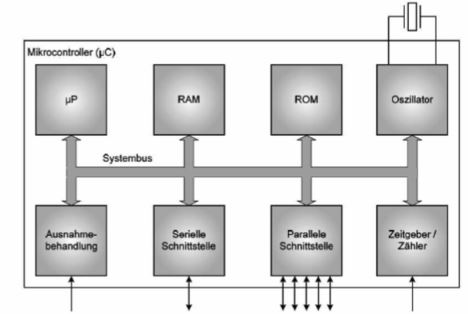
\includegraphics[width=\linewidth]{images/aufbauuC}
\end{minipage}

\begin{multicols}{2}
\subsubsection{Anwendungen}
\begin{minipage}{\linewidth}
\begin{itemize}
    \item Supercomputer
    \item Arbeits und Server-Rechnern
    \item Smartphones
    \item Navigationssysteme
    \item Digitalkameras
    \item Drucker
    \item ...
\end{itemize}
\end{minipage}

\begin{minipage}{\linewidth}
\subsubsection{Aufbau von uP-basierten Systemen}
\begin{itemize}
    \item Zentraleinheit CPU mit
    \begin{itemize}
        \item Rechenwerk ALU
        \item Steuerwerk CU
        \item Registersatz
    \end{itemize}
    \item Speicher
    \item Eingabe-/Ausgabe-Schnittsellen
\end{itemize}
\end{minipage}
\end{multicols}

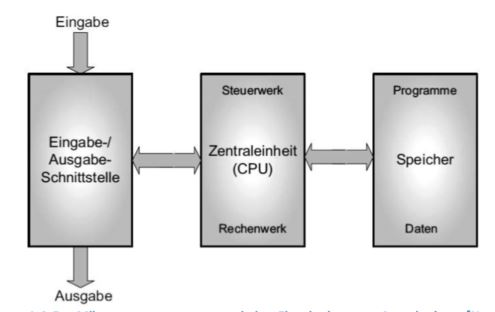
\includegraphics[width=0.5\linewidth]{images/aufbauuC1}
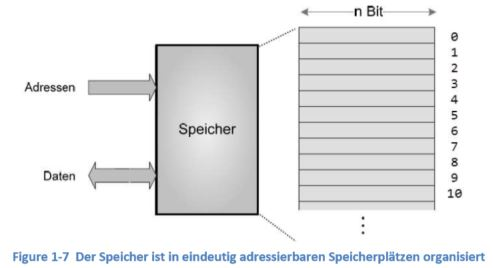
\includegraphics[width=0.5\linewidth]{images/aufbauuCspeicher}

\subsubsection{Havard vs Von Neumann Architektur}
\begin{multicols}{2}
    \begin{minipage}{\linewidth}
        \textbf{Harvard Rechnermodell}\\
        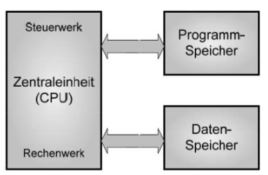
\includegraphics[width=0.6\linewidth]{images/HavardArchi}
    \end{minipage}
    
    \begin{minipage}{\linewidth}
        \textbf{von Neumann Rechnermodell}\\
        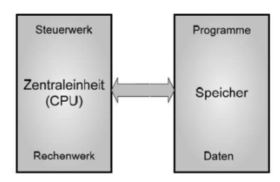
\includegraphics[width=0.6\linewidth]{images/NeumannArchi}
    \end{minipage}
\end{multicols}
\clearpage
%===================================
\subsubsection{Programmierung eins uP}
\begin{multicols}{2}
\begin{minipage}{\linewidth}
    Ein $\mu$ P kann durch individuelle Programmierung auf ganz unterschiedliche Art angepasst werden. \newline
    $\rightarrow$ entscheidend für die Durchdringung im Markt.\newline
    Ein Programm enthält in aufeinanderfolgender Anordnung die Maschinen-Befehle oder -Instruktionen für den $\mu$ P. Diese Maschiene-Befehle teilen der CPU mit, welche Operationen in welcher Reihenfolge und auf welche Daten angewendet werden sollen. \newline
    Die Befehlsfolge des Programms wird innerhalb der CPU vom Steuerwerk gesteuert und schrittweise ausgeführt. Dazu wird der aktuell zur bearbeitende Befehl durch einen Programmzähler (PC) im Speicher adressiert.\newline
    Der PC enthält laufend die Adresse der Speicherzelle des jeweiligen Befehls im Speicher.
\end{minipage}

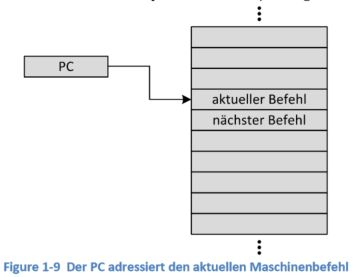
\includegraphics[width=\linewidth]{images/uPPC}
\end{multicols}
    
\subsubsection{Befehlsformate}
\begin{multicols}{2}
\begin{minipage}{\linewidth}
Die Art und Wirkung eines Befehls wird im Befehlswort (\textbf{OpCode}) codiert.
Darin sind neben der Operation auch die Operanden spezifiziert.
Die Codierung des Befehlswortes erfolgt abhängig vom $\mu$ P.
Der Maschinencode setzt sich aus einem OpCode und einem oder mehreren Operanden zusammen.
\end{minipage}

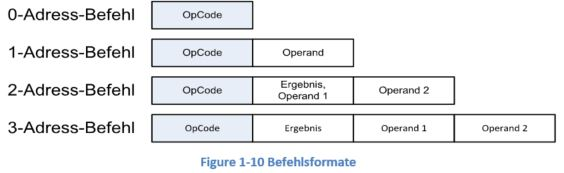
\includegraphics[width=\linewidth]{images/Befehlsformate}
\end{multicols}


\subsection{RISC vs CISC}
\begin{multicols}{2}
    \textbf{CISC}\newline
    Complex Instruction Set Computer
    \\
    \textbf{RISC}\newline
    Reduced Instruction Set Computer
\end{multicols}
\subsubsection{RISC-Rechner}
effizienter als CISC-Rechner
\begin{itemize}
    \item besteht aus einer kleinen Anz. von Befehlen mit wenigen Adressierungsarten
    \item Registersatz enthält eine grosse Anzahl von allg. verwendbaren Registern\newline
    General Purpose Register (GPR)
    \item Speicherzugriff erfolgt über spezielle Lade- und Speicher-Befehle
    \begin{itemize}
        \item Arithmetisch-logische Operationen arbeiten auf Registeroperanden
    \end{itemize}
    \item Pipeline-Architecture $\leftarrow$ Leistungssteigernde Architektur
    \item Eine grosse semantische Lücke entsteht bei der Übersetzung aus der Hochsprache
\end{itemize}

\subsubsection{u Architektur}
Beschreibt die architektonischen Details bei der Implementierung der $\mu$ P aus Sicht der Programmierer.
Dies umfasst die Beschreibung der Zentraleinheit (CPU), des Rechenwerks (ALU) und des Steuerwerks (CU).


\clearpage

\subsection{Hardware}
\begin{minipage}[t]{10cm}
	\subsubsection{Registersatz}
	Register sind schnelle Zwischenspeicher für \newline
	temporäre Daten im $\mu$ P.
\end{minipage}
\begin{minipage}[t]{0.5\linewidth}
	\subsubsection{Hardware- /Software-Schnitsttelle}
	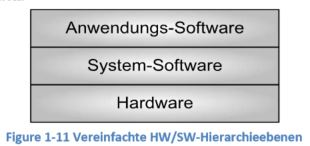
\includegraphics{images/HardwareSoftware}
\end{minipage}

\subsubsection{Taktfrequenz}
Das Taktsignal steuert die zeitliche Abfolge im $\mu$ P \newline
\begin{multicols}{2}
        \begin{minipage}{\linewidth}
    \[ f_{Takt}= \frac{1}{T_{takt}} \]
        \end{minipage}
    
    \begin{minipage}{\linewidth}
        $ \Uparrow $ Taktrate \-\ $ \Leftrightarrow $ \-\ $  \Uparrow  $Leistungsaufnahme \\
        Um Energie zu sparen ist es sinnvoll die Taktrate laufend anzupassen.\\
    \end{minipage}
\end{multicols}
\subsubsection{Leistungsaufnahme}
\begin{multicols}{2}
        \begin{minipage}{\linewidth}
\[ P_{Gate}= \frac{1}{2} \cdot C_{Last} \cdot V_{DD}^2\cdot f_{Takt} \]
    \end{minipage}
    
\begin{minipage}{\linewidth}
    $ P_{Gate} \qquad $Leistung pro CMOS Gate \newline
    $ C_{Last} \qquad $Lastkapazität\newline
    $ V_{DD}   \qquad $Versorgungsspannung\newline
    $ f_{Takt} \qquad $Taktfrequenz
\end{minipage}
\end{multicols}

\subsection{Software}
\begin{minipage}[b]{11cm}
	\subsubsection{Ablauf}
	\begin{itemize}
    	\item Der \textbf{Präprozessor} bereitet das Quellprogramm für den Compiler vor
    	\item Der \textbf{Compiler} übersetzt das Programm von einer Hochsprache in ein Assembly-Programm
    	\item Der \textbf{Binder} fasst verschiedene Dateien, die verschiebbaren Maschinencode enthalten, zu einem Programm zusammen.
    	\item Der \textbf{Loader} wandelt die verschiebbaren Adressen in absolute Adressen um und lädt sie in den Speicher des Systems.
	\end{itemize}
\end{minipage}
%
\begin{minipage}{0.5cm}
	\-\
\end{minipage}
%
\begin{minipage}{7cm}
	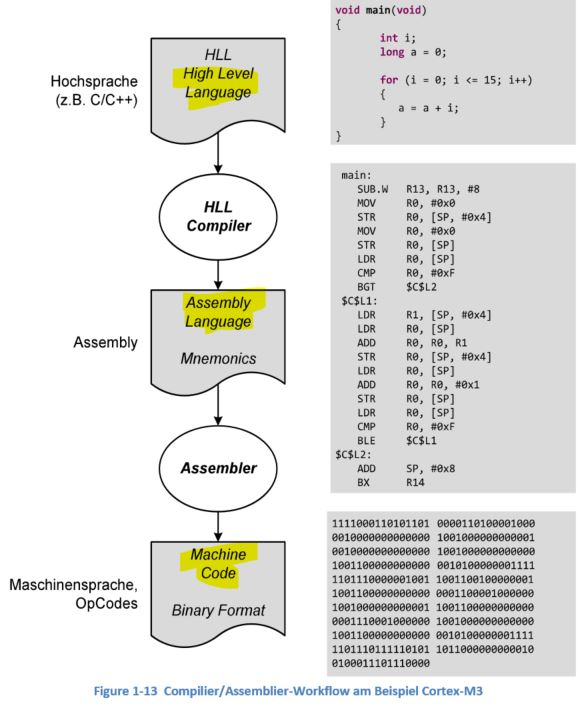
\includegraphics[width=\linewidth]{images/CompilerWorkflow}
\end{minipage}






















    
\clearpage
\section{V3}
\subsection{Halbleiter Speicher}
\begin{multicols}{2}
\textbf{Zentraler Speicher}
\begin{itemize}
    \item direkt am Bussystem angeschlossen
\end{itemize}
\textbf{Peripherer Speicher}
\begin{itemize}
    \item über I/O-Schnittstelle angeschlossen
\end{itemize}

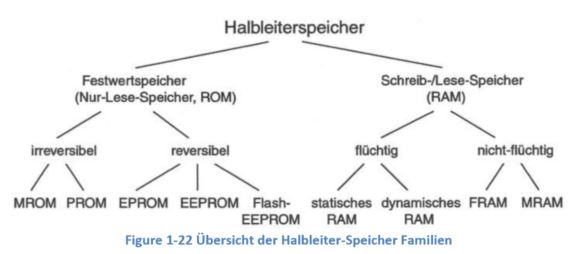
\includegraphics[width=10cm]{images/halbleiterfam}
\end{multicols}

\begin{multicols}{2}
\subsubsection{ROM-Festwertspeicher}
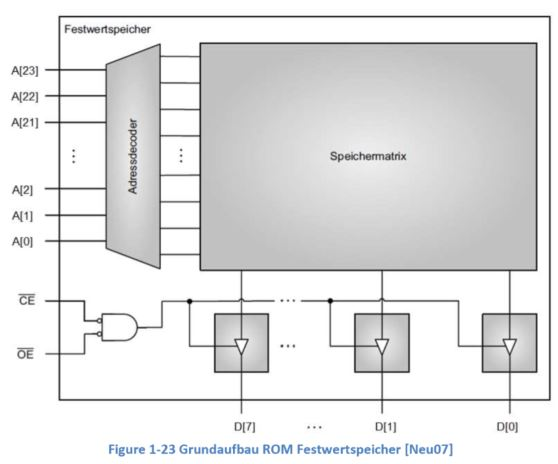
\includegraphics[width=8cm]{images/ROM}

\subsubsection{RAM-Speicher-/Lese-Speicher}
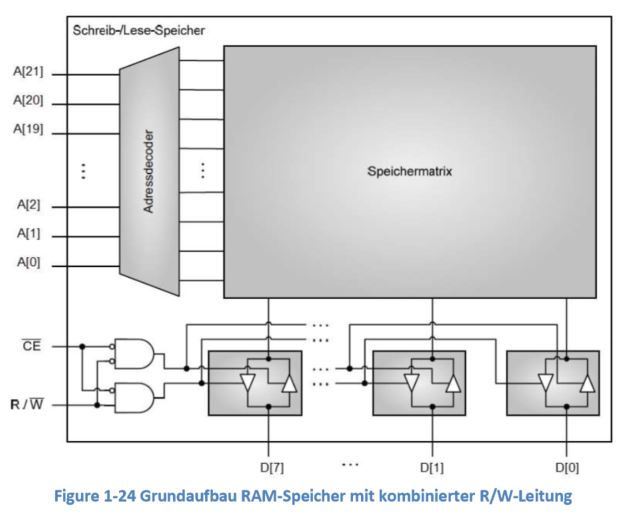
\includegraphics[width=8cm]{images/RAM}
\end{multicols}

\subsection{Speicherorganisation}
\begin{multicols}{2}
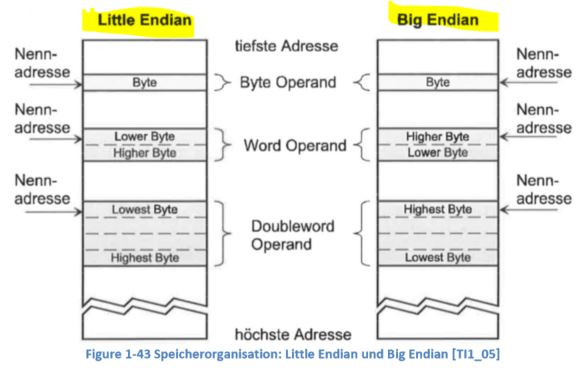
\includegraphics[width=8cm]{images/LittleBigEndian}

\subsubsection{I/O - Schnittstelle}
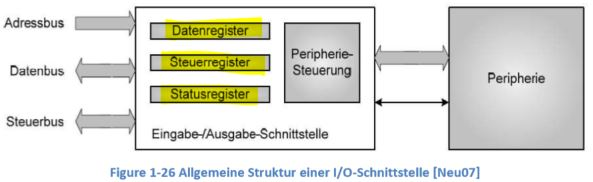
\includegraphics[width=8cm]{images/IOSchnittstelle}
\end{multicols}

\includegraphics{images/Speicherraumadressierung}
\section{Cortex}
\subsection{Cortex M Varianten}
\begin{multicols}{2}
\textbf{Cortex M0 und M0+}
    \begin{itemize}
        \item kleinster Vertreter der CortexFam
        \item Ersatz von 8Bit- uC
        \end{itemize}                     
 \textbf{Cortex M1}
    \begin{itemize}
        \item als Softcore Implementiert
        \item Vergleichbar mit Cortex-M0
    \end{itemize}
\end{multicols}
\begin{multicols}{2}
   \textbf{Cortex M3}     
     \begin{itemize}
         \item erster Vertreter der CortexFam
         \item 32 Bit Architektur
         \item ersetzt 8 \& 16 Bit uC
         \item Thumb ISA (Instruction Set Architecure)\newline
         Mix aus 16 und 32BIt langen anweisungen
     \end{itemize}   
               
   \textbf{Cortex M4} 
    \begin{itemize}
        \item vergleichbar mit M3 jedoch mit
        \qquad\item Digital Signal Processing (DSP)
        \qquad\item Floating Point Unit (FPU)
        \newline
      \end{itemize}  
\end{multicols}
\clearpage
\begin{multicols}{2}
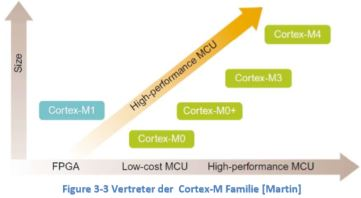
\includegraphics[width=\linewidth]{images/cortexmfam}

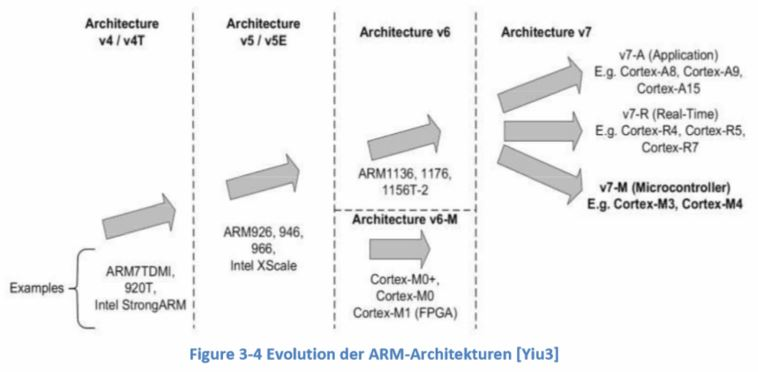
\includegraphics[width=\linewidth]{images/cortexmcomp}
\end{multicols}

\begin{multicols}{3}
    \textbf{Cortex-A}
    \begin{itemize}
        \item HighEnd Anwendungen und Betriebssysteme
        \item hohe Rechenleistung
        \item Chache Memory
    \end{itemize}
    
    \textbf{Cortex-R}
    \begin{itemize}
       \item Echtzeitfähigkeit
       \item hohe Zuverlässigkeit
       \item System on Chip (SOC) 
    \end{itemize}  
    
        \textbf{Cortex-M}
        \begin{itemize}
            \item Speziell für \mu C-Markt
            \item Low Cost, Low Energy
            \item System on Chip (SOC) 
          \end{itemize}             
\end{multicols}
\subsubsection{Vorteile der Cortex-M-Prozessoren}
\begin{itemize}
    \item Low Power
        \subitem < 200\mu A / MHz
    \item Performance
        \subitem >1.25 DMIPS / MHz
    \item Energy Efficiency
        \subitem low Power, high performance
    \item Code Density
        \subitem Thumb 2 Befehlssatz
    \item Interrupts
        \subitem 240 Interrupts
    \item Easy of Use, C Friedly
    \item Scalability
    \item Debug Features
    \item Software portability and Reusebility
    \item OS Support
    \item Choices (Derivers, Tools, OS,..)    
\end{itemize}























\clearpage
\section{V3}
\vspace{-0.5cm} 
    \begin{minipage}{9cm}
        \subsection{Halbleiter Speicher} 
        \textbf{Zentraler Speicher}
        \begin{itemize}
            \item direkt am Bussystem angeschlossen
        \end{itemize}
        \textbf{Peripherer Speicher}
        \begin{itemize}
            \item über I/O-Schnittstelle angeschlossen
        \end{itemize}
    \end{minipage}
    %
    \begin{minipage}{0.5cm}
    	\ \
    \end{minipage}
    %
    \begin{minipage}{9cm}
    	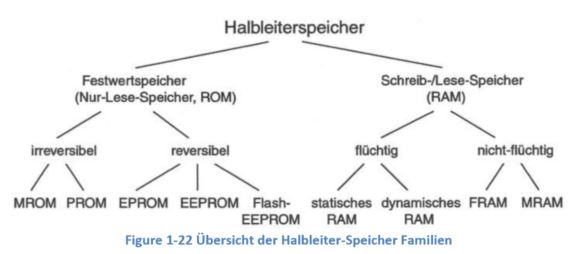
\includegraphics[width=9cm]{images/halbleiterfam}
    \end{minipage}
 
\begin{multicols}{2}
    \subsubsection{ROM-Festwertspeicher}
    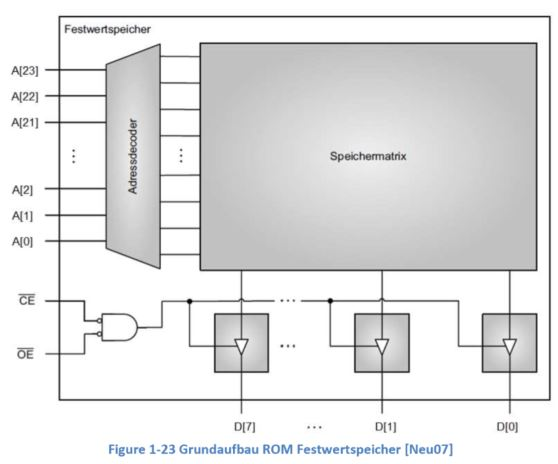
\includegraphics[width=8cm]{images/ROM}
    
    \subsubsection{RAM-Speicher-/Lese-Speicher}
    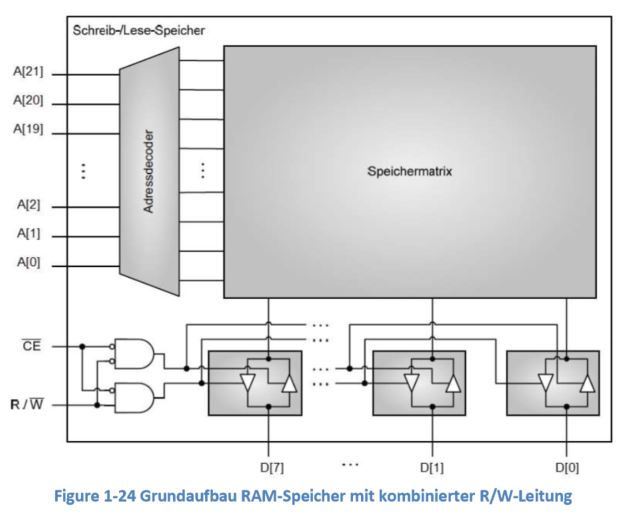
\includegraphics[width=8cm]{images/RAM}
\end{multicols}

\subsection{Speicherorganisation}
\begin{minipage}{9cm}
	\subsubsection{Little/Big Endian}
    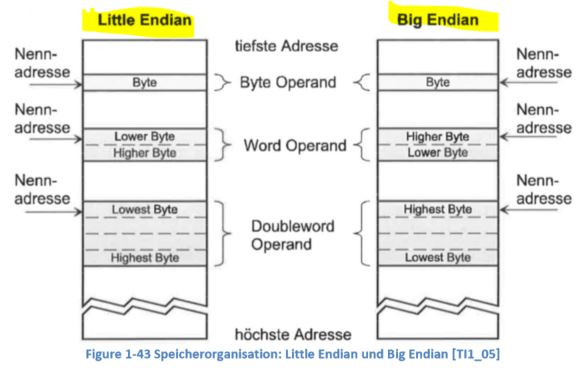
\includegraphics[width=8cm]{images/LittleBigEndian}
    
    Der ARM Cortex verwendet standardm"assig \textbf{Little Endian} f"ur die Speicherorganisation. 
\end{minipage}
%
\begin{minipage}{0.5cm}
	\-\
\end{minipage}
%
\begin{minipage}{9cm}
	 \subsubsection{I/O - Schnittstelle}
    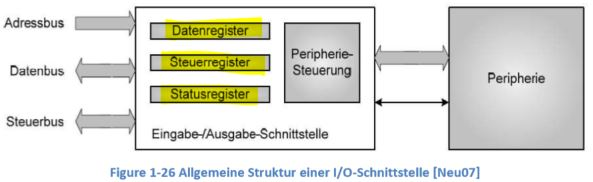
\includegraphics[width=8cm]{images/IOSchnittstelle}
    
    \textbf{Datenregister}
    \begin{itemize}
    	\item enthalten die zu verarbeitenden Daten
    \end{itemize}
    \textbf{Steuerregister}
    \begin{itemize}
    	\item dienen zur Konfiguration der Ein-/Ausgabe Schnittstelle
    \end{itemize}
    \textbf{Statusregister}
    \begin{itemize}
    	\item signalisieren den Zustand der Ein-/Ausgabe Schnittstelle
    \end{itemize}
\end{minipage}
 
\subsubsection{Speicherraumadressierung}
\begin{minipage}{11cm}
	\includegraphics[width=11cm]{images/Speicherraumadressierung}
\end{minipage}
%
\begin{minipage}{0.5cm}
	\-\
\end{minipage}
%
\begin{minipage}{7cm}
	\textbf{Isolierte Adressierung}
	\begin{itemize}
		\item Gesamter Adressraum steht verschiedener Bl"ocken zur Verf"ugung
		\item Bl"ocke werden mit einem Steuersignal ausgew"ahlt
	\end{itemize}
	\textbf{Memory-Mapped I/O (Cortex M3)}
	\begin{itemize}
		\item Verschiedene Bl"ocke werden in einen Adressraum eingebettet
		\item Ben"otigt eine Adresskodierung
	\end{itemize}
\end{minipage}

\newpage
\subsection{Busanschluss und Adressverwaltung}
Eine Adressverwaltung hat verschiedene Aufgaben zu erf"ullen:
\begin{itemize}
	\item Jede Adresse spricht nur einen einzigen Speicher- oder I/O-Baustein an.
	\item Adressraum m"oglichst gut ausn"utzen
	\item Adressr"aume von Speicherbausteinen m"ussen l"uckenlos aufeinander folgen.
	\item Jeder interne Speicherplatz bzw. jedes Register erscheint unter einer eigenen Adresse im Systemadressraum.
\end{itemize}

\subsubsection{Adresskodierung}
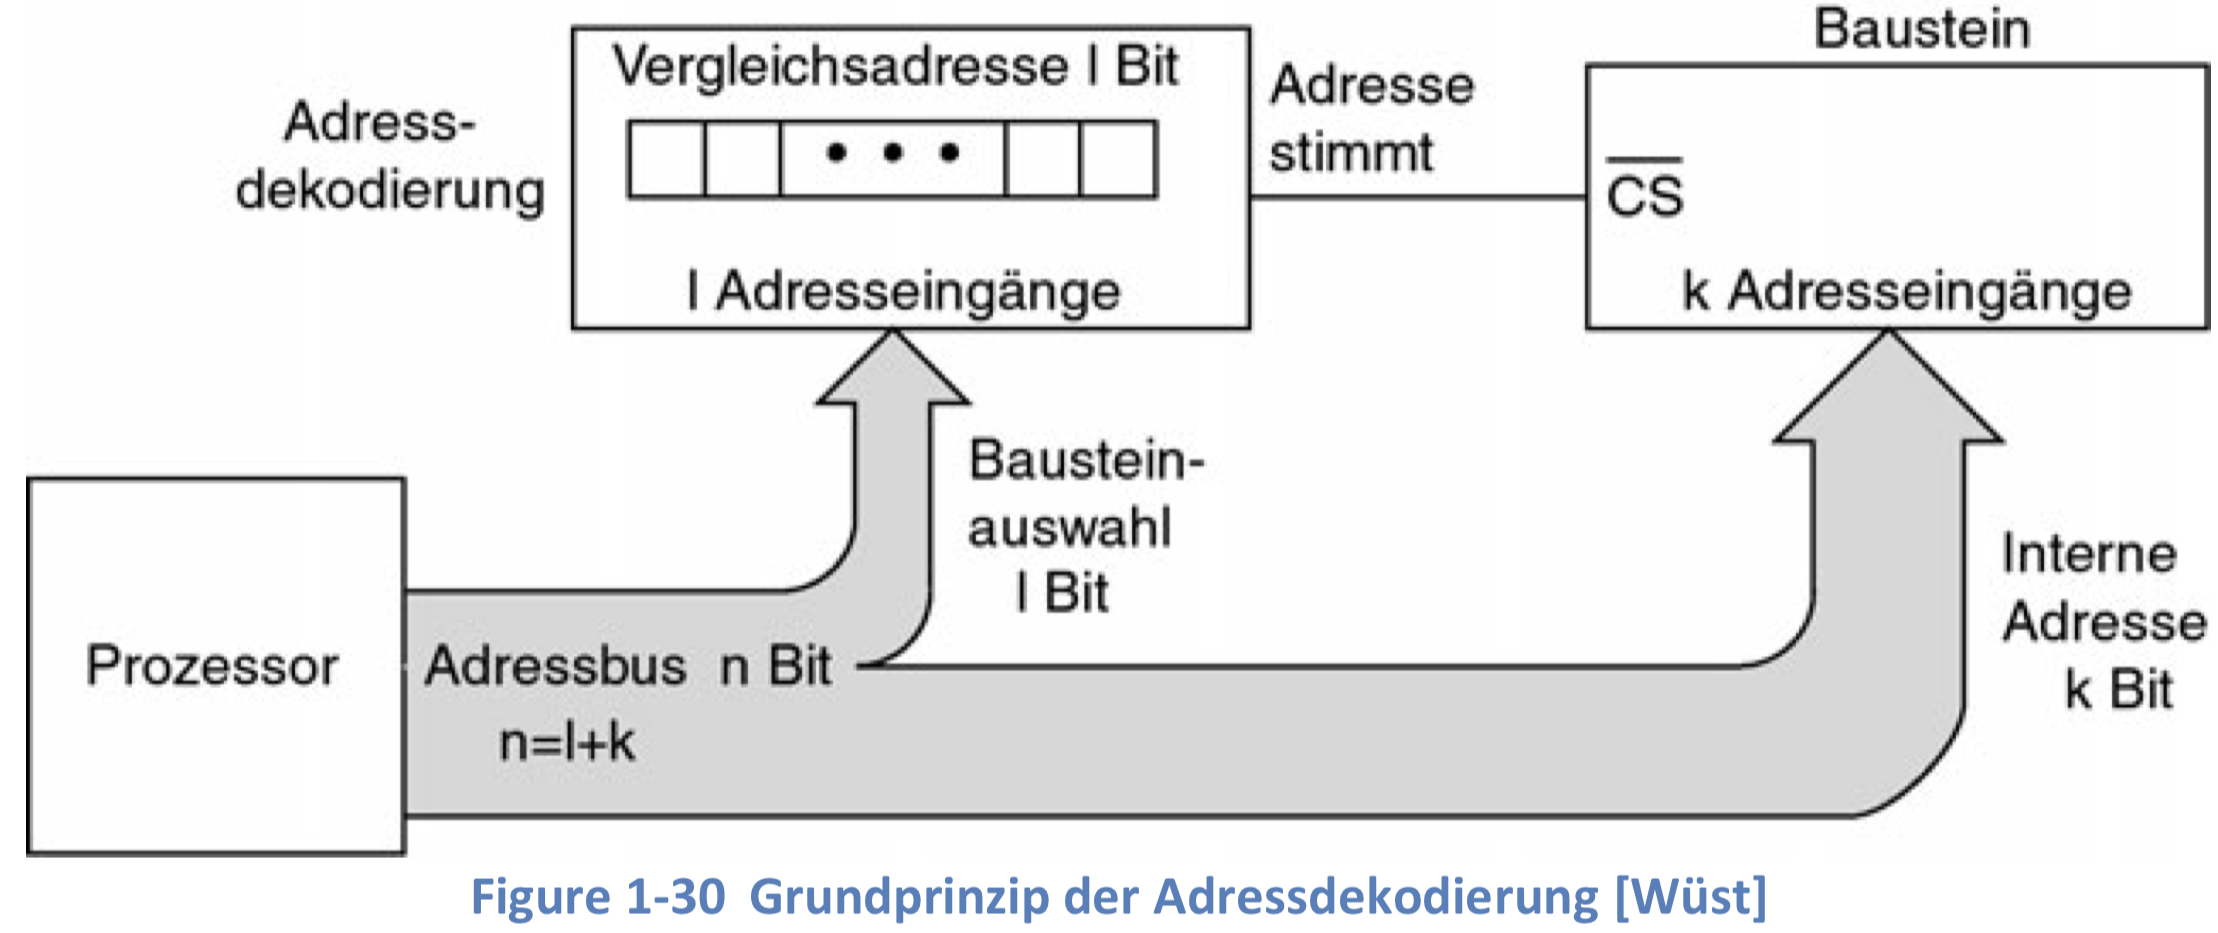
\includegraphics[width=14cm]{images/Adressverwaltung}\\
Der Kernpunkt der Adresskodierung ist die Teilung des Adressbuses. Dabei werden die \textit{k} niedrigsten Adressleitungen direkt an die Adresseing"ange des Bausteines gef"uhrt und dienen zur Auswahl des gew"unschten internen Speicherplatzes oder Registers. Die n"achstfolgenden \textit{l} Adressleitungen werden zur Adresskodierung auf einen Adressdekoder gef"uhrt.
\clearpage
%============================================























\clearpage
\section{V4}
\subsection{Cortex M Varianten}
\begin{multicols}{2}
    \textbf{Cortex M0 und M0+}
    \begin{itemize}
        \item kleinster Vertreter der CortexFam
        \item Ersatz von 8Bit- uC
    \end{itemize}                     
    \textbf{Cortex M1}
    \begin{itemize}
        \item als Softcore Implementiert
        \item Vergleichbar mit Cortex-M0
    \end{itemize}
\end{multicols}

\begin{multicols}{2}
    \textbf{Cortex M3}     
    \begin{itemize}
        \item erster Vertreter der CortexFam
        \item 32 Bit Architektur
        \item ersetzt 8 \& 16 Bit uC
        \item Thumb ISA (Instruction Set Architecure)\newline
        Mix aus 16 und 32Bit langen anweisungen
    \end{itemize}   
    
    \textbf{Cortex M4} 
    \begin{itemize}
        \item vergleichbar mit M3 jedoch mit:
        \subitem - Digital Signal Processing (DSP)
        \subitem - Floating Point Unit (FPU)
        \newline
    \end{itemize}  
\end{multicols}
\begin{multicols}{2}
    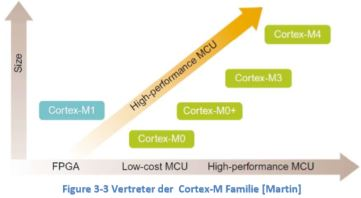
\includegraphics[width=\linewidth]{images/cortexmfam}
    
    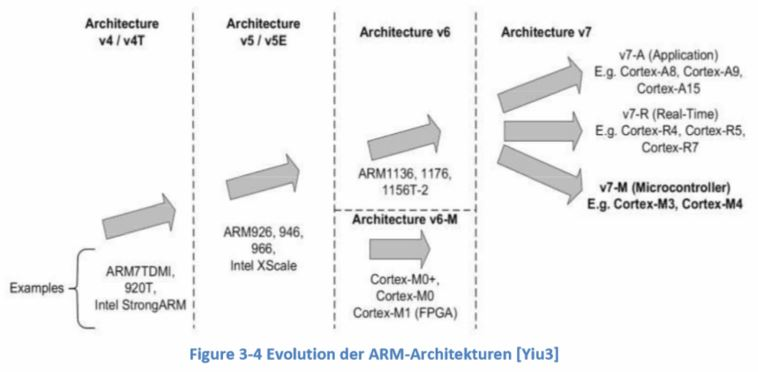
\includegraphics[width=\linewidth]{images/cortexmcomp}
\end{multicols}

\begin{multicols}{3}
    \textbf{Cortex-A}
    \begin{itemize}
        \item HighEnd Anwendungen und Betriebssysteme
        \item hohe Rechenleistung
        \item Chache Memory
    \end{itemize}
    
    \textbf{Cortex-R}
    \begin{itemize}
        \item Echtzeitfähigkeit
        \item hohe Zuverlässigkeit
        \item System on Chip (SOC) 
    \end{itemize}  
    
    \textbf{Cortex-M}
    \begin{itemize}
        \item Speziell für \mu C-Markt
        \item Low Cost, Low Energy
        \item System on Chip (SOC) 
    \end{itemize}             
\end{multicols}

\subsubsection{Vorteile der Cortex-M-Prozessoren}
\begin{multicols}{2}
    \begin{itemize}
        \item Low Power
        \subitem < 200\mu A / MHz
        \item Performance
        \subitem >1.25 DMIPS / MHz
        \item Energy Efficiency
        \subitem low Power, high performance
        \item Code Density
        \subitem Thumb 2 Befehlssatz
        \item Interrupts
        \subitem 240 Interrupts
        \item Easy of Use, C Friedly
        \item Scalability
        \item Debug Features
        \item Software portability and Reusebility
        \item OS Support
        \item Choices (Derivers, Tools, OS,..)    
    \end{itemize}
\end{multicols}
\clearpage 

\subsection{Cortex-M3/M4}
\begin{multicols}{2}
    \begin{itemize}
        \item Harvard Architecture
            \subitem \rightarrow  Zugriffe auf Instruktionen und Daten
            \subitem \qquad können gleichzeitig stattfinden
        \item Internal Bus Interconnect
            \subitem \rightarrow mehrere Bus-Interface 
        \item Nested Interrupt Controller \textbf{(NVIC)}
        \item Standart Timer \textbf{(SYSTICK)}\\
        \textbf{Optional:}
        \item Memory Protection Unit \textbf{(MPU)}
        \item Floating Point Unit \textbf{(FPU)}
    \end{itemize}
\end{multicols}

\subsection{System-Komponenten}
\begin{multicols}{2}
    \begin{minipage}{\linewidth}
        \subsubsection{NVIC}
        \begin{itemize}
            \item Non-Maskable Interrupt (NMI)
            \item Bis zu 240 externe Interrupts
            \item 8 bis 256 Prioritätslevel
        \end{itemize}
        \rightarrow ISR benötigt 12 Taktzyklen\newline
        Siehe auch:\nameref{NVIC} S\pageref{NVIC}\\
    \end{minipage}

    \begin{minipage}{\linewidth}
        \subsubsection{WIC (Wakeup Interrupt Controller)}
        Für die Umsetzung von Low-Power-Modes.\newline
        Dadruch kann 99\% der Cortex M3-Prozessoren im Low-Power-Bereich arbeiten.
        \newline
        \newline
        Ist mit dem NVIC verknüpft und holt den Prozessor aus diesem Modus heraus, um auf einen Interrupt reagieren zu können\\
    \end{minipage}
    
    \begin{minipage}{\linewidth}
        \subsubsection{FPU - (nur Cortex M4!)}
        Mit der FPU lassen sich IEEE754 Signal Precision Floating-Point Operationen in sehr wenigen Takten ausführen\\
    \end{minipage}
    
    \begin{minipage}{\linewidth}
        \subsubsection{MPU}
        \begin{itemize}
            \item ermöglicht Zugriffsregel für den Privilieged Access und User Programm Access zu definieren
            \item \rightarrow Wird eine Zugriffsrege verletzt erfolgt eine Exception-Regelung wodurch der Exceptrion Handler das Problem analysiert und ggf. beheben kann
            \item \rightarrow Ausserdem ist es möglich gewisse Bereiche als read-only zu deklarieren
        \end{itemize}
    \end{minipage}
\end{multicols}

\begin{multicols}{2}
    \begin{minipage}{\linewidth}
        \subsubsection{SYSTICK}
        \begin{itemize}
            \item 24-Bit Countdown-Timer mit automatischer Relaod-Funktion
            \item Wird für einen periodischen Interrupt verwendet
        \end{itemize}
        Wenn der Zähler den Wert 0x000000, wird dies dem NVIC signalisiert und  der Reload-Wert wird aus dem Reload-Register gelesen.
    \end{minipage}
    \\
    \newline
    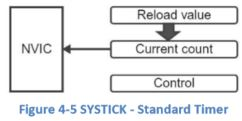
\includegraphics[width=6.5cm]{images/NVIC}\\
\end{multicols}
\clearpage
%============================================

\subsection{GNU-Tool-Chain Entwicklungsablauf}
\begin{multicols}{2}
    \begin{minipage}{\linewidth}
        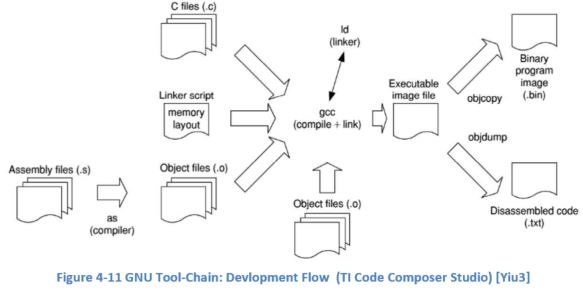
\includegraphics[width=\textwidth]{images/gnutoolchain}
        \begin{tabular}{|l|l|}
            \hline 
            \textbf{APSR}& Application Program Status Register \\ 
            \hline 
            \textbf{IPSR}& Interrupt Program Status Register \\ 
            \hline 
            \textbf{EPSR}& Execution Program Status Register \\ 
            \hline 
            \end{tabular}
        \subsubsection{SP-zugriffe(Assembler)}
        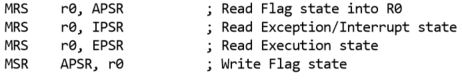
\includegraphics[width=\textwidth]{images/SPzugriffe}   
    \end{minipage}
    
    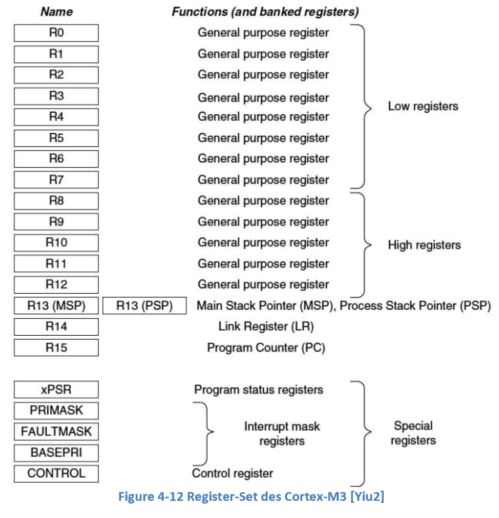
\includegraphics[width=0.5\textwidth]{images/gnutoolchain1}
\end{multicols}

\subsection{Programm Status Register}
\renewcommand{\arraystretch}{1.2}
\begin{minipage}{\linewidth}
    \begin{tabular}{|l|l|}
        \hline 
        \textbf{N}& Negativ \\ 
        \hline 
        \textbf{Z}& Zero  \\ 
        \hline 
        \textbf{C}& Carry/borrow  \\ 
        \hline 
        \textbf{V}& Overflow \\ 
        \hline 
        \textbf{Q}& Sticky saturation flag \\ 
        \hline 
        \textbf{ICI/IT}& Interrupt-Continauble Instruction(ICE) bits\\
                        & IF-THEN instruction status bit \\ 
        \hline 
        \textbf{T}& Thumb state, always 1; Trying to clear this bit will caus a fault exception \\ 
        \hline 
        \textbf{Exception number}& Indicates whiche exception the processor is handeling \\ 
        \hline 
    \end{tabular} 
\end{minipage}

\subsubsection{Q-Flag}
This flag is set to 1 if any of the following occurs:
\begin{itemize}
    \item Saturation of the addition result in a \textit{QADD or QDADD} instruction
    \item Saturation of the subtraction result in a \textit{QSUB or QDSUB} instruction
    \item Saturation of the doubling intermediate result in a \textit{QDADD or QDSUB} instruction
    \item Signed overflow during an \textit{SMLA<x><y> or SMLAW<y>} instruction
\end{itemize}
The Q flag is sticky in that once it has been set to 1, it is not affected by whether subsequent calculations saturate and/or overflow.\newline
\textbf{An example:}\newline
\textit{0x70000000 + 0x70000000} would become \textit{0xE0000000}, but since qadd is saturating, the result is saturated to \textit{0x7FFFFFFF} (the largest positive 32-bit integer) and the Q flag is set.
\clearpage
%===================================
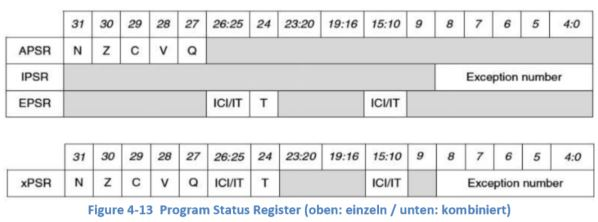
\includegraphics[width=19cm]{images/programstatusregister}

\subsection{Stack}
\begin{multicols}{2}
    \begin{minipage}{0.5\textwidth}
        \begin{itemize}
            \item Temporäre Zwischenspeicherung von Daten während der ausführung einer Funktion
            \item Übergabe von Informationen an Funktionen oder Subroutinen
            \item Speichern von lokalen Variabeln
            \item Erhalten von Prozessor-Status und Register-Werten, während Exceptions oder Interrupts ausgefüht werden
            \item PUSH-POP-Instruktionen werden ausgeführt
            \item LIFO-Prinzip(Last In, First Out)
        \end{itemize}
    \end{minipage}
    
    \begin{minipage}{0.5\textwidth}
        \subsubsection{Main-Stak-Pointer (MSP)}
        \begin{itemize}
            \item Standart Stack Pointer nach einem Reset
            \item Innerhalb von Exception-Interrupt-Handler wird immer der MSP benutzt!
            \end{itemize}
        \subsubsection{Prozesor-Stack-Pointer (PSP)}
        \begin{itemize}
            \item Alternativer Stackpointer
            \item Wird nur im Thread-Mode verwendet
            \subitem \rightarrow bei embedded OS-System
        \end{itemize}   
    \end{minipage}
\end{multicols}


















\clearpage
\section{V5}
\subsection{Data Alignment}
\begin{tabular}{|l|l|l|}
    \hline 
    1 Byte & 8 Bit  & Byte  \\ 
    \hline 
    2 Byte & 16 Bit & Half-Word \\ 
    \hline 
    4 Byte & 32 Bit & Word \\ 
    \hline 
    8 Byte & 64 Bit & Double-Word \\ 
    \hline 
\end{tabular} 

\subsubsection{Aligned-Unaligned Data}
\begin{multicols}{2}
    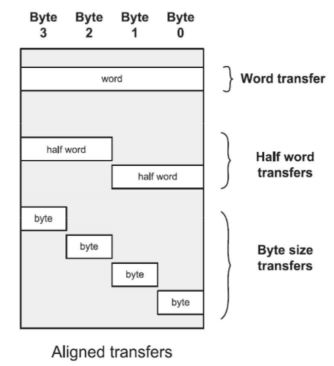
\includegraphics[width=0.5\textwidth]{images/alignedData}
    
    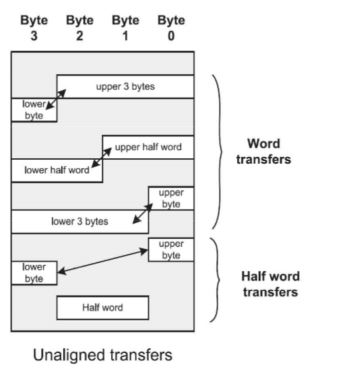
\includegraphics[width=0.5\textwidth]{images/unalignedData}
\end{multicols}
    \clearpage
\subsubsection{Bit-Banding}
\[\textbf{ BitBandAliasAddress = BitBandAliasBase + (MemoryAddres - BitbandRegionBase)* 32 + 4*BitNumber} \]
    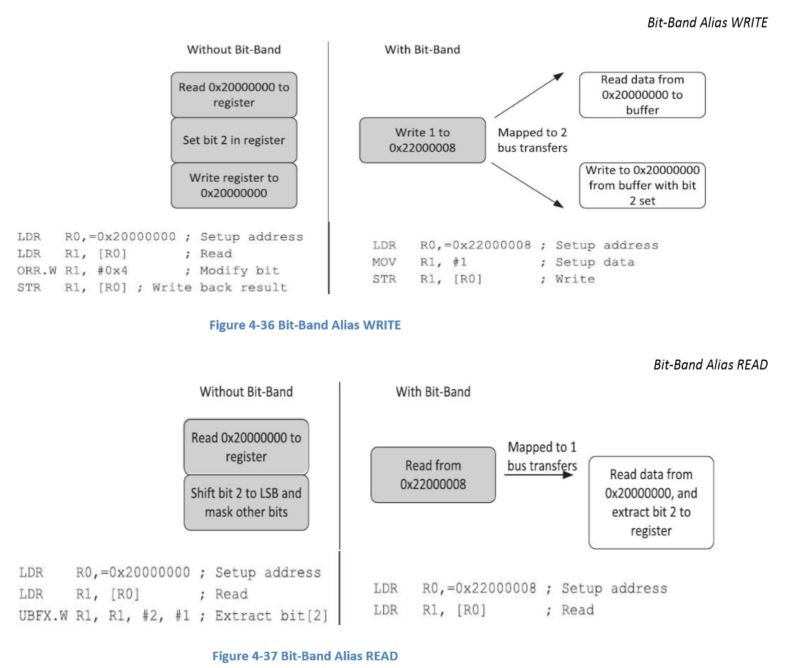
\includegraphics[width=\textwidth]{images/bitbanding}
\clearpage
\section{V6}
\begin{multicols}{2}
    \begin{minipage}{\linewidth}
        \subsection{Exceptions and Interrupts}\label{Exceptions}
        Der NVIC verarbeitet bis 240 IRQ und einen NMI\\
        \begin{tabular}{ll}
            normaler Programmablauf& \rightarrow Background  \\ 
            Exception-Handler& \rightarrow Foreground  \\ 
        \end{tabular} 
    \end{minipage}
    
    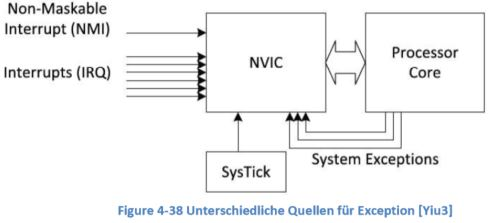
\includegraphics[width=\linewidth]{images/NVICExcp}
\end{multicols}
Exception-Handler für Interrupts werden als Interrupt Service Routine (ISR) bezeichnet.

\subsection{Reset und Reset-Sequenzen}
\subsubsection{Reset}
Es gitb 3 Arten von Reset:\\
\begin{tabular}{ll}
    \textbf{Power-on Reset}  & Resettet den gesammten \mu C, auch alle Preripherien und Debug-Komponenten \\ 
    \textbf{System Reset}    & Resettet nur den Prozessor und die Periferien, aber nicht die Debug-Komponenten \\ 
    \textbf{ Processer Reset}& Resettet nur den Prozessor\\
\end{tabular}

\subsubsection{Reset Sequenz}
     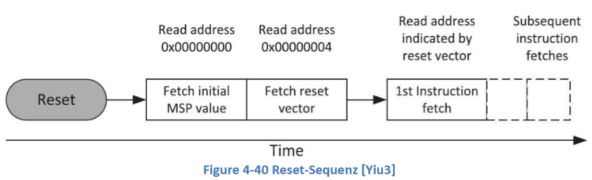
\includegraphics{images/resetsequenz}
\subsection{Spezial-Register}     
Register um Exceptions ein oder auszuschalten:\\
\textbf{\rightarrow PRIMASK,FAULTMASK,BASEPRI}
\begin{multicols}{2}
    \subsubsection{PRIMASK}
    \begin{itemize}
        \item 1-bit Register
        \item Wenn das aktiv ist, werden NMI-Interrupts erlaubt
        \subitem \rightarrow alle anderen Interrupts werden überdeckt
        \subitem \rightarrow Default-Wert= 0, also deaktiviert
    \end{itemize}
    
    \subsubsection{FAULTMASK}
    \begin{itemize}
        \item 1-bit Register
        \item Wenn das aktiv ist, werden nur noch NMI-Interrups akzeptiert.\newline
        alle anderen Interrupts und Exceptioln-Handlings werden deaktiviert
        \subitem \rightarrow Default-Wert = 0
    \end{itemize}
\end{multicols}

\subsubsection{BASEPRI}
\begin{itemize}
    \item Register das bis zu 8 Bits enthalten kann
    \item definiert eine Prioritätsstufe
    \item Hohe Stufe = Hohe Priorität
    \item Wenn das gesetzt wird, werden alle Interrupts mit gleicher oder tieferer Stufe deaktiviert
\end{itemize}

\subsubsection{Control-Register}
Das Kontroll-Register definiert:
\begin{enumerate}
    \item Die Auswahl zwischen MSP (Main-SP) und PSP (Process-SP)
    \item Die Zugriffsstufe und Thread-Mode
    \subitem (Ob Privilegd oder unprivilegd)
\end{enumerate}
\begin{multicols}{2}
    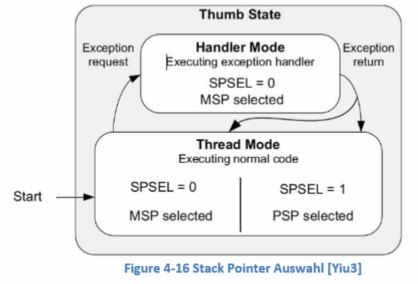
\includegraphics[width=\linewidth]{images/StackPointerAuswahl}
    
    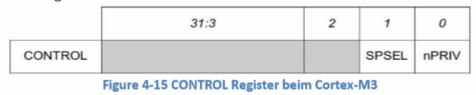
\includegraphics[width=\linewidth]{images/controlRegister}
\end{multicols}
\clearpage
\section{V7 (ausgefallen)}
\section{V8}
\begin{minipage}[t]{9cm}
	\subsection{Cortex M3 Instruction Set}
	\subsubsection{Thumb-2 Instruction Set}
    \begin{tabular}{l l}
        Ziel:&-Erhöht die Code-Dichte\\
            &  -Mehr Leistung\\ 
        Cortex M3 Processor:  & 1.25 DMIPS / MHz\\ 
    \end{tabular} 
    
\subsection{Instruction Pipelining}
                  Mit Pipelining bearbeitet der Cortex-M Prozessor zur gleichen Zeit drei Befehle - jeweils um einen Takt versetzt.\\
     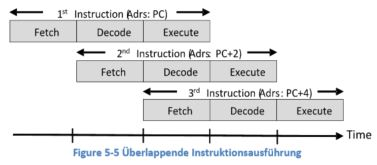
\includegraphics[width=9cm]{images/pipelining}\\
     \begin{tabular}{m{1.5cm} m{6.5cm}}
        Fetch:& 16-Bit Instruktion aus Programmspeicher laden\\
        Decode:& Vorangehende Instruktion decodieren\\ 
        Execute:& Nochmals vorangehende Instruktion ausf"uhren\\
    \end{tabular} 
    Bei einem Sprung im Programmcode muss eine Pipeline komplett geleert werden, da die sequentielle Reihenfolge je nach Konstellation nicht korrekt ist.
\end{minipage}
%
\begin{minipage}[t]{0.5cm}
	\-\
\end{minipage}
%
\begin{minipage}[t]{9cm}
	\subsection{Logikstruktur des Cortex-M Prozessor}
        \begin{tabular}{ll} 
            Sourceoperanden:& Rn, Rm \\ 
            Destinationsoperand:& Rd  \\ 
            MAC:& Memory Access Calculator\\

        \end{tabular} \\
        Ein \textit{Barrel-Shifter} vereinfacht Berechnungen,\newline
        da Multiplikationen einfacher realisiert werden können.\\
        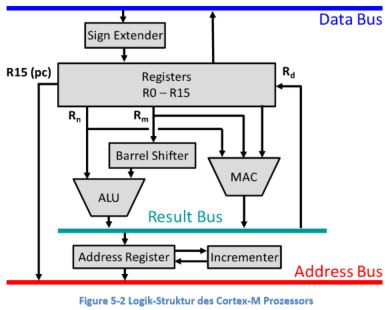
\includegraphics[width=9cm]{images/logikstrukturcortex}
        
        Das 32-Bit breite Programm-Status-Register (xPSR) enth"alt die Flags. Das xPSR gliedert sich in drei verschiednen Darstellungen, je nach aktuellem Prozessorstatus als: \textit{Application-Program Register (APSR), Interrupt-Program Status Register (IPSR)} oder \textit{Execution-Program Status Regsiter (EPSR)}.\\
        Die wichtigsten Flags (N, Z, C, V) sind die vier h"ochsten Bits des APSR, welche die Basis f"ur bedingte Verzweigungen darstellen.
\end{minipage}

\subsection{Anwendungen}
    \begin{minipage}{6cm}
       \subsubsection{Cortex-M0/M0+ / M1}  
        - einfaches I/O Handling 
    \end{minipage}
    %
    \begin{minipage}{0.25cm}
    	\-\
    \end{minipage}
    %
    \begin{minipage}{6cm}
        \subsubsection{Cortex-M3}   
        - Komplexe Datenverarbeitung\newline
        - anspruchsvolle Applikationenen
    \end{minipage}
    %
    \begin{minipage}{0.25cm}
    	\-\
    \end{minipage}
	%
    \begin{minipage}{6cm}
        \subsubsection{Cortex-M4}   
       -  DSP-Funktionalität\newline
       -  Floating Point Support
    \end{minipage}

\newpage
\subsection{Software Development Prozess}
\begin{minipage}{9.5cm}
	Die Umsetzung von Hochsprachen Source-Code in Assembly-Language und weiter in den bin"aren OpCode des jeweiligen Prozessors ist ein komplexer, mehrstufiger Prozess. Im ersten Durchgang  baut der Assembler eine Symboltabelle auf, welche Informationen "uber sogenannte \textit{programmer-defined Identifiers} enth"alt (z.B. Adressen von Sprungmarken, Subroutinen, Variablen, I/O-Port Registern, usw.). W"ahrend des zweiten Durchgangs benutzt der Assembler diese Informationen, um die einzelnen Assembler-Instruktionen zu vervollst"andigen. Erst in einem weiteren Teilschritt der Assemblierung werden die bin"aren OpCode ermittelt.
\end{minipage}
%
\begin{minipage}{0.5cm}
	\-\
\end{minipage}
%
\begin{minipage}{8.5cm}
	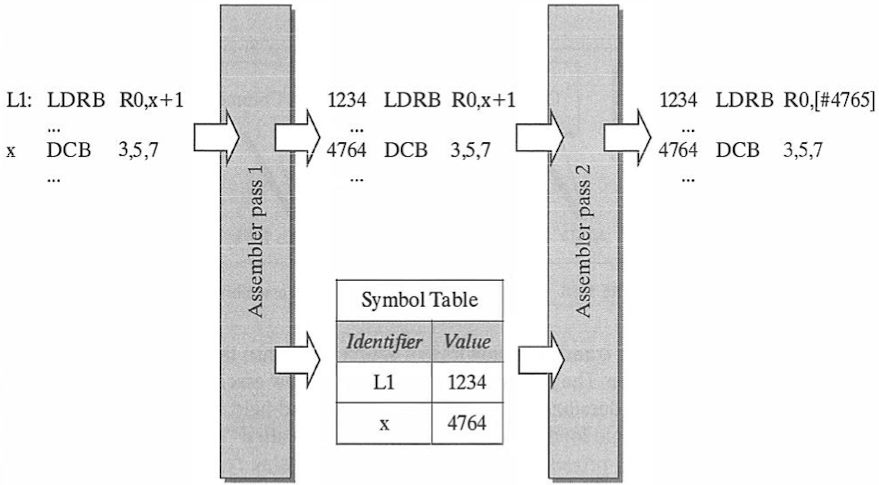
\includegraphics[width=8.5cm]{images/SoftwareDevelopmentProzess}
\end{minipage}

\subsection{Assembly-Language Syntax}
\begin{tabular}{llll}
    \textbf{Lable}  &\textbf{OpCode}  &\textbf{Operand}  & \textbf{Comment} \\ 
    L1  & ADD &R0,R1,\#5    & Replace R0 by sum of R1 and 5 \\ 
    FUNC& MOV &R0,\#100     & this sets R0 to value 100 \\  
        & BX  &LR           & this is a function return\\
\end{tabular} 
\begin{tabular}{|ll}
    \textbf{Lable}  & optional  \\ 
    \textbf{OpCode} & spezifiziert den Befehl \\ 
    \textbf{Operand}& Parameter  \\ 
    \textbf{Comment}&  optionale Beschreibung\\ 
\end{tabular} 
\\
\begin{multicols}{2}
    \begin{minipage}{\linewidth}
        \subsection{Unified Assembler Language (UAL)}
        Syntax für ARM und Thumb Instructionen.\\
        Die meisten Instruktionen arbeiten mit Registern\\
        \textbf{BSP}\newline
        \begin{tabular}{lll}
            MOV&R2,\#100  &;R2=100,Direkte Zuweisung  \\ 
            LDR&R2,[R1]   &;R2= den Wert von R1  \\ 
            ADD&R2,R0     &;R2=R2+R0  \\ 
            ADD&R2,R0,R   &;R2=R0+R1  \\ 
        \end{tabular} 
    \end{minipage}
    
    \begin{minipage}{0.8\linewidth}
        \subsubsection{Register List}
        \begin{tabular}{lll}
            Norm. Form&{reglist}  &;{R1,R2...Rn}  \\ 
            PUSH& {LR} & ;save LR on stack\\ 
            POP&  {LR}&  ;remove from stack; place in LR\\  
            PUSH& {R1-R3,LR} & ;save R1,R2,R3; return address\\  
            POP& {R1-R3,PC} &;restore R1,R2,R3 and return \\ 
        \end{tabular} 
    \end{minipage}
\end{multicols}

\subsection{Addressing}
 \subsubsection{Immediate Adressing}
\begin{minipage}{10cm}
        Der Datenwert ist unmittelbar in der Instruktion erhalten. Daher kein zusätzlicher Speicherzugriff erforderlich\newline
        Form: \# imm\newline
        \colorbox{lightgray}{
        \begin{tabular}{lll}
             MOV & R0,\# 100&;R0=100, immediate addressing \\ 
        \end{tabular} }
\end{minipage}
%
\begin{minipage}{0.5cm}
	\-\
\end{minipage}
%
\begin{minipage}{8cm}
	 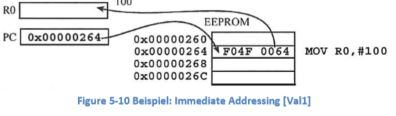
\includegraphics[width=8cm]{images/immediateAddressing}    
\end{minipage}  

\subsubsection{Indirect Addressing}
\begin{minipage}{10cm}
        Bei der \textit{Indirect Addressing} Modes sind die Daten im Memory. Ein Register enth"alt irgendwie einen Zeiger auf diese Daten. Nach der \textit{Fetch}-Phase , bei welcher die Instruktion aus dem Programmspeicher gelesen wird,
        sind noch einer oder mehrere Speicherzugriffe erforderlich um die Daten zu lesen oder zu schreiben.\newline
        Form: [Rn]\newline
        \colorbox{lightgray}{
        \begin{tabular}{lll}
            LDR & R0,[R1]&;R0=value pointed to by R1 \\ 
        \end{tabular} }\\
        \textbf{R1 wird nicht verändert}
\end{minipage}
%
\begin{minipage}{0.5cm}
	\-\
\end{minipage}
%
\begin{minipage}{8cm}
	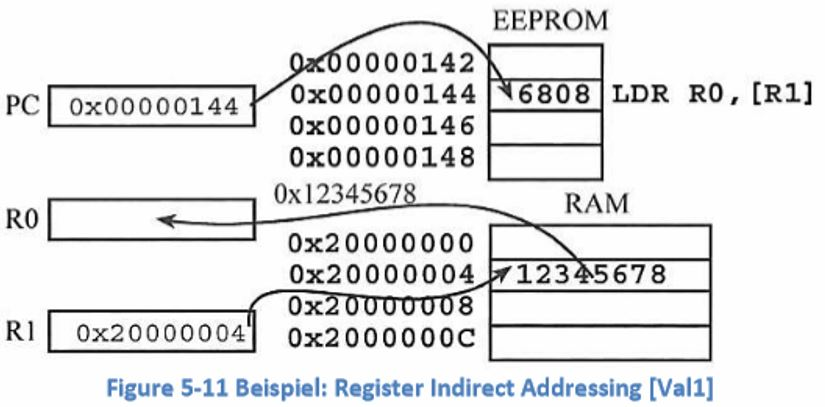
\includegraphics[width=8cm]{images/indirectAddressing}    
\end{minipage}

\subsubsection{Register Addressing with Displacement}
\begin{minipage}[b]{10cm}
        Dasselbe, nur wird hier dem Wert R0 noch \# 4 hinzugefügt\newline
        R1 bleibt weiterhin unverändert.\newline
        Form: [Rn,\# imm]\newline
        \colorbox{lightgray}{
        \begin{tabular}{lll}
            LDR & R0,[R1,\# 4]&;R0=word pointed to by R1+4 \\ 
        \end{tabular} }\\
\end{minipage}
%
\begin{minipage}{0.5cm}
    	\-\
\end{minipage} 
%
\begin{minipage}{8cm}
    	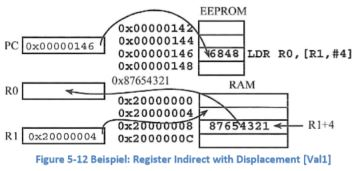
\includegraphics[width=8cm]{images/AddressingDisplacment}    
\end{minipage}

\subsubsection{Register Indirect with Index}
Form: [Rn,Rm]\newline
\colorbox{lightgray}{
\begin{tabular}{lll}
   LDR &R0,[R1,R2]  &;R0= word pointed to by R1+R2 \\ 
\end{tabular} }

\subsubsection{Register Indirect with shifted Index}
Form: [Rn,Rm,LSL \# imm]\newline
\colorbox{lightgray}{
\begin{tabular}{lll}
    LDR&R0,[R1,R2;LSL \#2]  &;R0= word pointed to by R1+4*R2  \\ 
\end{tabular} }

\subsubsection{Register Indirect with Pre-index}
Form: [Rn,\# offset]!\newline
\colorbox{lightgray}{
\begin{tabular}{lll}
   LDR & R0,[R1,\#4]! &;first R1=R1+4, then R0= word pointed to by R1  \\ 
\end{tabular} }

\subsubsection{Register Indirect with Post-index}
Form: [Rn],\# offset\newline
\colorbox{lightgray}{
\begin{tabular}{lll}
    LDR& R0,[R1],\#4  &;R0= word pointed to by R1, then R1=R1+4  \\ 
\end{tabular} }

\subsubsection{PC-relativ}
PC wird als Pointer verwendet.
Form: lable\newline
\begin{tabular}{lll}
    B   &Location   &;jump to Location\\ 
    BL  &Subroutine &;call Subroutine, Rücksprungadresse wird gespeichert\\ 
\end{tabular} 

\subsubsection{Speicher- und I/O-Zugriffe}
\begin{minipage}{10cm}
    Es benötigt immer zwei Instruktionen um auf Daren im RAM oder I/O zuzugreifen.
    $\rightarrow$ PC-Relative Addressierung wird verwendet
    \begin{enumerate}
        \item Erstellt Zeuger auf das Objekt
        \item Greift über den Zeiger Indirekt auf den Speicher zu
    \end{enumerate}
    \colorbox{lightgray}{
    \begin{tabular}{lll}
        LDR   &R1,Count   &;R1 points to variable Count\\ 
        LDR   &R0,[R1]    &;R0= value pointed to by R1\\ 
    \end{tabular} }
\end{minipage}
%
\begin{minipage}{0.5cm}
	\-\
\end{minipage}
%
\begin{minipage}{8cm}
	\includegraphics[width=\linewidth]{images/AddressingRAM}   
\end{minipage}






















\clearpage
\section{V8}
\subsection{Stack Push und Pop}
\begin{multicols}{2}
 \begin{minipage}{3cm}
     PUSH \qquad {R0}\newline
     PUSH \qquad {R1}\newline
     PUSH \qquad {R2}\newline
     POP \qquad {R3}\newline
     POP \qquad {R4}\newline
     POP \qquad {R5}\newline
 \end{minipage}
 \begin{minipage}{\linewidth}
    \includegraphics[width=1.5\linewidth]{images/stackpushpop}  
        \end{minipage}
\end{multicols}

\subsubsection{Generelle Regeln bei der Verwendung des Stacks}
\begin{multicols}{2}
\begin{enumerate}
    \item Funktionen sollten die gleiche Anzahl Push und Pop Befehle aufweusen
    \item Stackzugriffnur inerhalb des allozierten Bereichs
    \item Es sollte nicht über den SP auf den Stack geschrieben oder gelesen werden
    \item Stack sollte zuerst den SP dekrementieren und erst dann die Daten ablegen
    \item Stack sollte die Daten zuerst lesen und erst dann den SP inkrementieren
\end{enumerate}
    \includegraphics[width=0.8\linewidth]{images/allocatedStack}  
\end{multicols}
\subsection{Shift and Rotate}
\includegraphics[width=0.8\linewidth]{images/shiftandrotate} 
\clearpage
\section{V9}
\subsection{C/C++ Strukturen Umsetzen}
\subsubsection{Entscheidung treffen}
In Assembler-Sprache ist eine Entscheidung praktisch immer in einem 2-Stufigen Ablauf umgesetzt.
\begin{itemize}
    \item Benötigte Flags ermitteln
    \item Zugehörige bedingte Sprünge ausführen
\end{itemize}

\textbf{Ablauf}\newline
\vspace{-0.5cm}
\begin{enumerate}
    \item Vergleich: Zwei Werte werden subtrahiert, dabei wird nur auf die Flags geschaut.
    \item Anhand der Flags werden dann die bedingten Sprünge ausgeführt
\end{enumerate}















\clearpage
\section{V11}
\subsection{Subroutinen}
\includegraphics[width=0.8\linewidth]{images/subroutinen} 

\subsection{Architecure Producer Call Standart (AAPCS)}
\subsubsection{Regeln}
\begin{itemize}
    \item Bei Funktionsaufrufen werden die Register \textbf{R0-R3} als \textbf{Parameter} an eine C-Funktion verwendet
    \item Die Funktionen müssen die Inhalte der Register \textbf{R4-R11}(falls benutzt) während der Ausführung sichern, um sie am Ende wieder rekonstruieren
    \item Der \textbf{Rückgabewert} einer Subroutine (8-bit, 16-bit,32-bit) wird in den \textbf{Registern R0} übertragen. Handelt es sich um einen 64-bit Rückgabewert, so sind die unteren 32-bit im Register R0 und die oberen 32-bit im Register R1 übertragen
    \item Mit PUSH und POP wird immer eine \textbf{gerade Anzahl von Registern auf dem Stack} gelegt bzw. vom Stack eine \textbf{8-byte Alignment} auf dem Stack einzuhalten
\end{itemize}
\clearpage
\section{V12, Serielle Schnittstelle}
\subsection{Grundlagen}
\subsubsection{Serielle vs. Parallele Daten"ubertragung}
\begin{minipage}{12cm}
	Bei einem seriellen Kommu nikationskanal werden die einzelnen Datenbits sequenziell hintereinander "uber eine Signalleitung "ubertragen. Im Gegensatz dazu k"onnen bei einem parallel Kommunikationskanal mehrere Datenbits auf einmal transferiert werden. Sowohl bei der seriellen wie auch bei der parallelen "Ubertragung ist dabei immer eine bestimmte Bit-"Ubetragungszeit $t_{bit}$ einzuhalten.
	
	Bei seriellen Kommunikationskan"alen werden allgemein zwei unterschiedliche Metriken unterschieden, die \textit{Bit Rate} und die \textit{Baud Rate}.
	
	Die \textit{Bit Rate} sagt aus, wie viele \textit{bits-per-second} oder \textit{bts} "uber den Datenkanal transferiert werden k"onnen.
	
	Die \textit{Baud Rate} sagt aus, wie viele sogennante \textit{Symbols} sich in einer Sekunde "uber den Datenkanal transferieren lassen. Ist jedes Symbol durch ein Bit repr"asentiert spricht man von einer \textit{Dualen Codierung} (Bit/s = bps $\equiv$ Baud)
\end{minipage}
%
\begin{minipage}{0.5cm}
	\-\
\end{minipage}
%
\begin{minipage}{6cm}
	\includegraphics[width=6cm]{images/serielle-parallel_grundlagen}
\end{minipage}

\subsubsection{Parallel-Seriell Umsetzung}
Der Mikroprozessor verarbeitet die Daten intern in aller Regel parallel. F"ur die serielle Daten"ubertragung ist daher eine koordinierte Parallel-Serien-Wandlung in eine daf"ur vorgesehenen I/O-Port erforderlich.
	\begin{center}
		\includegraphics[width=12cm]{images/seriell_parallel}
	\end{center}
	
\subsubsection{Aufbau von Datenkan"alen}Kommunikatiosnkan"ale k"onnen auf verschiedene Arten implementiert werden. So k"onnen drahtgebundene Kan"ale beispielsweise als \textit{Single-Ended} oder als \textit{Differential Link} umgesetzt werden.\\
	
	\begin{minipage}[t]{9cm}
		\textbf{Single Ended (a)}\\
		Bei einer Single-Ended Verbindung werden einzelne, getrennte Signalleitungen ben"otigt, sowie eine Referenzleitung mit Ground-Potenzial
	\end{minipage}
	%
	\begin{minipage}[t]{0.5cm}
		\-\
	\end{minipage}
	%
	\begin{minipage}[t]{9cm}
		\textbf{Differential Link (b)}\\
		Bei einer Differential Verbindung wird der Datenlink durch eine Differenzspannung zwischen zwei zusammengeh"orenden Signalleitungen V(+) und V(-) repr"asentiert. Dies ist deutlich robuster als Single-Ended. F"ur eine serielle Differential Datenschnittstelle gen"ugen insgesamt drei Leitungen.
	\end{minipage}
	
	\begin{center}
		\includegraphics[width = 16cm]{images/diff_link}
	\end{center}

\newpage
\subsubsection{Simplex, Half- und Full-Duplex}
Datenkan"ale werden mit \textit{Simplex, Half-Duplex} oder \textit{Full-Doplex} bezeichnet, je nach Art der Konektivit"at.

		\textbf{Simplex}\\
		Ein Simplex serieller Kanal "ubertr"agt permanent in nur einer Richtung, "uber eine dedizierte Verbindung. An einem Ende des Kommunikationskanals arbeitet ein
			Transmitter, w"ahrend auf der anderen Seite ein Receiver steht. Simplex Kan"ale haben keine M"oglichkeit, den Empfang der Daten zu quittieren.
		\begin{center}
			\includegraphics[width=12cm]{images/Simplex_serial}
		\end{center}
		

		\textbf{Half-Duplex}\\
		Ein Half-Duplex serieller Kanal verf"ugt ebenfalls nur "uber eine einzige Verbindung. Diese erlaubt jedoch eine beidseitige Kommunikation, aber nur in einer Richtung zur gleichen Zeit. Auf beiden Seiten des Kommunikationskanals steht ein serieller Transceiver, der sowohl als Sender wie auch als Empf"anger arbeiten kann. Wird die "Ubertragungsrichtung ge"andert, so mu"ussen die beiden Transceiver ihre Betriebsart wechseln. Das Umschalten der Datenrichtung erfordert klare Regeln auf beiden Seiten, um beispielsweise ein gleichzeitiges Senden zu vermeiden.
		\begin{center}
			\includegraphics[width=12cm]{images/half_duplex}
		\end{center}
		
	 
	 	\textbf{Full-Duplex}\\
	 	Full-Duplex serielle Kan"ale verf"ugen "uber zwei separate Datenlinks; einer um Daten zu senden und ein anderer um Daten zu empfangen. Damit ist eine gleichzeitige Kommunikation in beide Richtungen m"oglich. Auf beiden Seiten des Kommunikationskanals steht ein serieller Transceiver, der zeitgleich als Sender und Empf"anger arbeitet.
	 	\begin{center}
			\includegraphics[width=12cm]{images/full_duplex}
		\end{center}

\newpage
\subsection{Synchrone Daten"ubertragung}
Synchrone serielle Kan"ale werden dadurch gekennzeichnet, dass Sender und Empf"anger auf das gleiche Clock-Signal synchronisiert sind $\Rightarrow$ zus"atzliche Clock-Leitung. Synchrone Kan"ale arbeiten "ublicherweise in einer \textit{Master/Slave-Beziehung}.\\
	\begin{center}
		\includegraphics[width=12cm]{images/synch_full_duplex}
	\end{center}
	
\subsubsection{Daten"ubertragung}
Beim der synchronen seriellen Datenkanal werden die Daten typischerweise in Bl"ocken mit variabler L"ange "ubertragen. Parallel dazu erfolgt die "Ubertragung der Clock Information. Dabei ist wichtig, dass Sender und Empf"anger auf die gleiche Flanke Daten "ubernehmen.

Im folgenden Bild ist exemplarisch eine ganze Message mit drei Data Packets (Datagrams) dargestellt: Das Synchronisationszeichen (Sync) kennzeichnet als Header den Beginn eines zusammengeh"orenden Data Pakets. Grunds"atzlich wird nach jedem Datenblock (Body) das Zeichen ETB (End of Transmission Block) als Footer "ubertragen. Das Ende der gesamten Message wird durch ein EOT (End of Transmission) gekennzeichnet. Das ETB kann vor einem EOT je nach Protokoll entfallen.
	\begin{center}
		\includegraphics[width=12cm]{images/synch-serielle-data-bsp}
	\end{center}

\subsection{Asynchrone Daten"ubertragung}
Beim asynchronen seriellen Datenkanal laufen auf der Sender- und Empf"angerseite zwei unabh"angige Clock-Generatoren. Dabei m"ussen diese auf die selbe Baud-Rate eingestellt werden. 
	\begin{center}
		\includegraphics[width=12cm]{images/asynch_serial.png}
	\end{center}

Auf die fallende Datenflanke des Datenframes wird der jeweilige Clock-Generator synchronisiert. Dabei haben Datenpakete folgenden Aufbau:\\
	\begin{minipage}{11cm}
		\includegraphics[width=11cm]{images/datenframe-uart}\\
		Datenframe einer UART Schnittstelle (7-Bit, Odd Parity)
	\end{minipage}
	%
	\begin{minipage}{0.5cm}
		\-\
	\end{minipage}
	%
	\begin{minipage}{7cm}
		Die beteiligten Kommunikationsschnittstellen ben"otigen folgende Informationen um ihre Interfaces auf den asynchronen seriellen Bitstrom abzustimmen:
		\begin{itemize}
			\item Baudrate = $\frac{1}{t_{bit}}$
			\item Anzahl Daten-Bits (5 bis 8)
			\item Parity Information (Even / Odd / none) Das Paritybit erg"anzt immer auf \textit{Odd} oder \textit{Even}.
			\item Anzahl Stop-Bit (1 / 1.5 / 2)
		\end{itemize}
	\end{minipage}\\

Aus den Informationen der Kommunikationsschnittstelle l"asst sich zudem die Nutzdatenrate bestimmen.
	\begin{equation*}
		Nutzdatenrate = \frac{\#Databit \cdot Baudrate}{\#Startbit + \#Databit + \#Paritybit + \#Stopbit} \cdot \frac{1 Byte}{8 Bit}
	\end{equation*}
	
\newpage
\subsubsection{Datenflusssteuerung}
Bei der seriellen Kommunikation muss oft der Datenfluss gesteuert werden. Dies ist zum Beispiel dann dringend notwendig, wenn empf"angerseitig der Datenpuffer voll wird und ein Daten"uberlauf droht. Dieser Zustand muss an den Datensender signalisiert werden. $\Rightarrow$ HW- und SW-Handshake\\

	\begin{minipage}[t]{9cm}
		\textbf{Hardware Handshaking}\\
		Mit Hardware-Signalen teilen sich die Kommunikationspartner gegenseitig mit, ob sie bereit sind weitere Daten aufzunehmen oder nicht.
		\begin{center}
			\includegraphics[width=5cm]{images/HW-handshake}\\
			\textit{RTS (request to send), CTS (clear to send)}
		\end{center}
	\end{minipage}	
	%
	\begin{minipage}[t]{0.5cm}
		\-\
	\end{minipage}
	%
	\begin{minipage}[t]{9cm}
		\textbf{Software Handshaking}\\
		Beim Software Handshaking kommen anstelle von zus"atzlichen Handshake-Leitungen zwei extra f"ur diesen Zweck reservierte ASCII-Zeichen zur Anwendung:
		\begin{itemize}
			\item \textbf{XON} ASCII DC1 0x11
			\item \textbf{XOFF} ASCII DC3 0x13
		\end{itemize}
		\begin{center}
			\includegraphics[width=5cm]{images/SW-handshake}
		\end{center}
	\end{minipage}
\subsection{Standardisierte serielle Interfaces}
\includegraphics[width=7cm]{images/uebertragungsraten_seriellen_schnittstellen}
\includegraphics[width=11cm]{images/uebersicht-serielle-schnittstellen}
\clearpage
\section{V13}
\subsection{Allgemeiner Ablauf von Exceptions und Interrupts}
\begin{minipage}{0.4\linewidth}
Interrupts werden in der Regel von der umgebenen Peripherie oder externen Input-Pins generiert und als Ereigniss der CPU-Infrastruktur signalisiert, welche dann eine Handler-Routine einschalten.\\
\textbf{Siehe} \nameref{Exceptions} Seite: \pageref{Exceptions}
\end{minipage}
\begin{minipage}{0.6\linewidth}
\includegraphics[width=\linewidth]{images/interruptablauf} 
\end{minipage}
\includegraphics[width=1\linewidth]{images/NVICExcp1} 
\clearpage
\section{V14}
\subsection{Spezielle Eigenschaften des NVIC}\label{NVIC}
\begin{minipage}{9cm}
	Alle Cortex-M Prozessoren enthalten einen \textit{Nested Vectored Interrupt Controller (NVIC)} f"ur das Interrupt-Handling. Neben den klassischen HW-initiierten Interrupts (IRQ) gibt es eine ganze Anzahl von Exceptions, die vom NVIC ebenfalls gehandhabt werden. Dazu geh"oren z.B. Fault Exceptions, NMI Software-Interrupts (SVC), SysTick Timer, usw.
\end{minipage}
%
\begin{minipage}{0.5cm}
	\-\
\end{minipage}
%
\begin{minipage}{9cm}
	\includegraphics[width=9cm]{images/nvic-cortex-m3} 
\end{minipage}

\subsection{Cortex-M3 Exceptions und Priority-Levels}
\begin{minipage}{9cm}
	Der erste Eintrag in der Vektor-Tabelle (Address-Offset: 0x00) enth"alt immer den Initialwert f"ur den Main Stack Pointer (MSP). Darauf folgt die Einsprung-Adresse f"ur den Reset-Handler. Durchl"auft der Cortex-M seine Reset-Sequenz, so werden diese beiden Eintr"age in den MSP bzw. in den PC geladen. Die n"achsten Eintr"age in der Vektor-Tabelle sind f"ur den Nonmaskable Interrupt (NMI), sowie vier verschiedene Faults reserviert. Weiter oben in der Vektor-Tabelle folgen die
		Adresseintr"age f"ur die weiteren System Exception-Handler.
\end{minipage}
%
\begin{minipage}{0.5cm}
	\-\
\end{minipage}
%
\begin{minipage}{9cm}
	\includegraphics[width=9cm]{images/NVICExcp1} 
\end{minipage}

\vspace{10pt}
\begin{minipage}[t]{9cm}
	\textbf{Usage Fault}\\
	Ein Usage Fault tritt auf, wenn der auszuf"uhrende Application-Code im Cortex-M3 zu einem un"uberwindbaren Fehler f"uhrt. Eine typische Ursache ist beispielsweise, wenn der Prozessor einen ung"ultigen OpCode auszuf"uhren versucht. Weitere Ursachen f"ur einen Usage Fault k"onnte eine Division durch Null sein.\\
	
	\textbf{Bus Fault}\\
	Ein Bus Fault wird ausgel"ost, wenn ein Fehler in der AHB-Bus Matrix erkannt wird. M"ogliche Gr"unde f"ur einen Bus Fault k"onnte eine falscher Memory-Bereich oder eine falsche Gr"osse f"ur einen Datentransfer sein.
\end{minipage}
%
\begin{minipage}[t]{0.5cm}
	\-\
\end{minipage}
%
\begin{minipage}[t]{9cm}
	\textbf{Memory Manager Fault}\\
	Die Memory Protection Unit (MPU) kann in den folgenden F"allen einen Memory
	Manager Fault ausl"osen:\\
	- Accessing an MPU region with the wrong privilege level\\
	- Writing to a read-only region\\
	
	\textbf{Hard Fault}\\
	Ein Hard Fault kann auf zwei Arten auftreten: (1) Wenn ein Bus Fault tritt auf, w"ahrend dem die Vektor-Tabelle gelesen wird. (2) Der Hard Fault wird durch die Eskalationen eines anderen, nicht behandelten Faults aktiviert.
\end{minipage}

\newpage
\subsubsection{Exception-Priority}
\begin{minipage}{9cm}
	Bei den Cortex-M Prozessoren kann individuell festgelegt werden, ob eine Exception zugelassen oder nicht zugelassen werden soll. Dazu wird der aktuelle Priority Level mit der konfigurierten Priority der Exception gegeneinander verglichen. Eine h"oher priorisierte Exception (kleinerer Priority Level) kann eine Exception mit tieferer Priorit"at (gr"osserer Priority Level) unterbrechen. Dieses \textit{preemptive} Verhalten
	wird allgemein als \textbf{Nested Exception/Interrupt Szenario} bezeichnet.\\

Das Priority-Level kann abh"angig vom Modell bis zu 8 Bit gross sein, und kann mit der \textit{Group-Priority} in die \textit{Preempt-Priority} und die \textit{Sub-Priority} aufgeteilt werden. $\Rightarrow$ Festlegung der Anzahl Priority-Level pro Gruppe
\end{minipage}
%
\begin{minipage}{0.5cm}
	\-\
\end{minipage}
%
\begin{minipage}{9cm}
	\includegraphics[width=9cm]{images/group-priority}
\end{minipage}


\vspace{10pt}
\begin{minipage}[t]{9cm}
	\textbf{Preempt-Priority}\\
	Legt fest ob ein Interrupt erfolgen kann, wenn bereits ein anderer Interrupt-Handler am laufen ist.
\end{minipage}
%
\begin{minipage}[t]{0.5cm}
	\-\
\end{minipage}
%
\begin{minipage}[t]{9cm}
	\textbf{Sub-Priority}\\
	Wird verwendet, wenn zwei Exceptions der selben Preempt Priority gleichzeitig auftreten. In solchen F"allen wird zuerst die Exception mit der h"oheren Sub-Priority (tieferer numerischer Wert) bearbeitet.
\end{minipage}

\subsubsection{Interrupt-Pending and Activation}
\begin{center}
	\includegraphics[width=15cm]{images/interrupt-pending}
\end{center}

\subsubsection{Tail Chaining}
Wenn eine Exception auftritt während bereits eine anderen Exception-Behandlung mit gleicher oder höherer Priorität läuft, so wird die neue Exception hinten angestellt. Nach Abschluss des laufenden Exception Handlers, kann die CPU sofort den neuen Exception Request behandeln

\subsubsection{Late arrival}
Wenn der Prozessor einen auftretenden Exceptionrequest akzeptiert, dann startet er die Stacking-Sequenz. Kommt während dem Stacking eine weitere Exception mit höherer Priorität hinzu, so kann diese Late-Arrival-Exception noch bevorzugt behandelt werden.

\subsubsection{POP Preemption} 
Diese Funktion stellt gewissermassen eine Umkehrung des Late-Arrivals dar. Wenn eine Exception Request während dem Unstacking auftritt, so wird das Unstacking abgebrochen, und sofort VectorFetch und Instruction Fetch für den neuen Request durchgeführt. $\rightarrow$ Geschwindigkeitsoptimierung\\


\clearpage
\section*{Anhang}
\subsection*{Glossar,Abkürzung}
    \includegraphics[width=0.75\linewidth]{images/glossar}  

\end{document}
